%% This is file `elsarticle-template-1-num.tex',
%%
%% Copyright 2009 Elsevier Ltd
%%
%% This file is part of the 'Elsarticle Bundle'.
%% ---------------------------------------------
%%
%% It may be distributed under the conditions of the LaTeX Project Public
%% License, either version 1.2 of this license or (at your option) any
%% later version.  The latest version of this license is in
%%    http://www.latex-project.org/lppl.txt
%% and version 1.2 or later is part of all distributions of LaTeX
%% version 1999/12/01 or later.
%%
%% The list of all files belonging to the 'Elsarticle Bundle' is
%% given in the file `manifest.txt'.
%%
%% Template article for Elsevier's document class `elsarticle'
%% with numbered style bibliographic references
%%
%% $Id: elsarticle-template-1-num.tex 149 2009-10-08 05:01:15Z rishi $
%% $URL: http://lenova.river-valley.com/svn/elsbst/trunk/elsarticle-template-1-num.tex $
%%

%%\documentclass[preprint, 12pt]{elsarticle}
\documentclass[final,5p,times,twocolumn]{elsarticle}
\usepackage{multirow}
\usepackage{multicol}
\usepackage{pdflscape}
\usepackage{caption}
\usepackage{subcaption} 
\usepackage{amsmath}
\usepackage[singlelinecheck=false]{caption}
\usepackage[latin1]{inputenc}
\usepackage{tikz}
\usetikzlibrary{shapes,arrows,calc}
\usepackage{float}
\captionsetup[table]{labelfont=bf, labelformat=simple, labelsep=newline, skip=0pt}
\usepackage[english]{babel}
\usepackage{blindtext}
\usepackage{tabularx}
\usepackage{longtable}
\captionsetup[subtable]{labelformat=simple, labelsep=colont}
\captionsetup[figure]{labelfont=bf, labelformat=simple, justification=centering}

%% Use the option review to obtain double line spacing
%% \documentclass[preprint,review,12pt]{elsarticle}

%% Use the options 1p,twocolumn; 3p; 3p,twocolumn; 5p; or 5p,twocolumn
%% for a journal layout:
%% \documentclass[final,1p,times]{elsarticle}
%% \documentclass[final,1p,times,twocolumn]{elsarticle}
%% \documentclass[final,3p,times]{elsarticle}
%% \documentclass[final,3p,times,twocolumn]{elsarticle}
%% \documentclass[final,5p,times]{elsarticle}
%% \documentclass[final,5p,times,twocolumn]{elsarticle}

%% if you use PostScript figures in your article
%% use the graphics package for simple commands
%% \usepackage{graphics}
%% or use the graphicx package for more complicated commands
%% \usepackage{graphicx}
%% or use the epsfig package if you prefer to use the old commands
%% \usepackage{epsfig}

%% The amssymb package provides various useful mathematical symbols
\usepackage{amssymb}
%% The amsthm package provides extended theorem environments
%% \usepackage{amsthm}

%% The lineno packages adds line numbers. Start line numbering with
%% \begin{linenumbers}, end it with \end{linenumbers}. Or switch it on
%% for the whole article with \linenumbers after \end{frontmatter}.


%% natbib.sty is loaded by default. However, natbib options can be
%% provided with \biboptions{...} command. Following options are
%% valid:

%%   round  -  round parentheses are used (default)
%%   square -  square brackets are used   [option]
%%   curly  -  curly braces are used      {option}
%%   angle  -  angle brackets are used    <option>
%%   semicolon  -  multiple citations separated by semi-colon
%%   colon  - same as semicolon, an earlier confusion
%%   comma  -  separated by comma
%%   numbers-  selects numerical citations
%%   super  -  numerical citations as superscripts
%%   sort   -  sorts multiple citations according to order in ref. list
%%   sort&compress   -  like sort, but also compresses numerical citations
%%   compress - compresses without sorting
%%
%% \biboptions{comma,round}

% \biboptions{}


\journal{the chair of supply chain management}

\begin{document}

\begin{frontmatter}

%% Title, authors and addresses

%% use the tnoteref command within \title for footnotes;
%% use the tnotetext command for the associated footnote;
%% use the fnref command within \author or \address for footnotes;
%% use the fntext command for the associated footnote;
%% use the corref command within \author for corresponding author footnotes;
%% use the cortext command for the associated footnote;
%% use the ead command for the email address,
%% and the form \ead[url] for the home page:
%%
%% \title{Title\tnoteref{label1}}
%% \tnotetext[label1]{}
%% \author{Name\corref{cor1}\fnref{label2}}
%% \ead{email address}
%% \ead[url]{home page}
%% \fntext[label2]{}
%% \cortext[cor1]{}
%% \address{Address\fnref{label3}}
%% \fntext[label3]{}

\title{Hybrid selective simulated annealing heuristic for the team orienteering problem with time windows and service time dependent profits}

%% use optional labels to link authors explicitly to addresses:
%% \author[label1,label2]{<author name>}
%% \address[label1]{<address>}
%% \address[label2]{<address>}

\author{Pascal Rauprecht}
\address{European University Viadrina, Frankfurt (Oder), Germany}



\begin{abstract}
%% Text of abstract
%\blindtext[2]
In this paper, an extension of the team orienteering problem with time windows, the team orienteering problem with time windows and service time dependent profits (TOPTWSTDP), is introduced. In the TOPTWSTDP, a number of vehicles have the goal to find the best possible route potentially visiting multiple locations to maximize their collected profits. Doing this, they are limited by specific time windows of each location, only allowing them to visit after the opening time and before the closing time. In contrast to the traveling salesman problem, not all locations have to be visited. The vehicles are also obliged to return to their depot before a preset time. The contribution of this paper to the TOPTWSTDP class is twofold. A mathematical model is provided to solve small instances exactly using mixed integer programming. In case of larger instances, an exact solution is not feasible due the significant required computational times. To accommodate this, a hybrid selective simulated annealing (HSSA) heuristic is proposed, which is delivering results of high quality in a reasonable amount of time. Since the TOPTWSTDP is a new problem class, benchmark solutions do not exist yet. Due to this reason, this paper is providing multiple benchmark results of the HSSA heuristic.
%\begin{enumerate}
%\item Part: Description of TOPTWSTDP
%\item Part: Description of Paper
%\end{enumerate}
\end{abstract}

\begin{keyword}
Team orienteering problem with time windows \sep Meta-heuristics \sep Service-time dependent profit
%% keywords here, in the form: keyword \sep keyword

%% MSC codes here, in the form: \MSC code \sep code
%% or \MSC[2008] code \sep code (2000 is the default)

\end{keyword}

\end{frontmatter}

%%
%% Start line numbering here if you want
%%

%% main text
\section{Introduction}
In the team orienteering problem with time windows (TOPTWSTDP) and service time dependent profits, a number of locations, also called vertices, and one depot is given. The locations have a time window in which they can be serviced. A predefined number of vehicles have the goal to visit locations in such a way, that the total collected profit is optimal after finishing their routes. The vehicles start not earlier than the opening time window and finish not later than the closing time window of the depot. In contrast to the team orienteering problem with time windows (TOPTW)\cite{Vansteenwegen:2008pet}, the time a vehicle is spending in one location influences the profit it is collecting in that vertex. The vehicle has to stay in a location for a specific minimum time. After a certain maximum time, which can vary depending on the location, the vehicle is not collecting profit anymore. \\
The main contribution of this paper is a metaheuristic approach to solve the TOPTWSTDP. The hybrid selective simulated annealing heuristic (HSSA) is decomposing the problem into two subproblems. The overarching subproblem is a routing problem, in which a decision has to be made on which location has to be visited by which vehicle. After making this decision the second problem represents a scheduling problem, where a determination of the starting time and the length of the stay in each location for each vehicle has to be conducted.\\ 
For the scheduling problem, dynamic programming was chosen to solve this problem exactly, since the number of possible states and stages are deterministic.\\
For the routing problem, the simulated annealing heuristic from Lin and Yu \cite{Lin:2012sa} was chosen and adapted to cope with the new requirement of service time dependent profits. It was also slightly extended, since Lin and Yu \cite{Lin:2012sa} always took the whole sequence of locations into considerations in their heuristic, whereas the HSSA heuristic is only considering a subset of locations for a certain number of iterations. \\
The remainder of the paper is organized as follows: In Section 2 a literature review is presented. In Section 3 the mathematical model for the TOPTWSTDP is provided. Section 4 describes the HSSA heuristic including the dynamic programming approach to solve the scheduling problem and the selective simulated annealing approach to solve the routing problem. Section 5 presents experimental results, where results and computing times of the mixed integer programming are compared with the results from the HSSA heuristic. Conclusions and further research will be discussed in Section 6. \\

\section{Literature Review}
The orienteering problem (OP), a special case of the TOPTW, in which time windows are either non-existent or not relevant and the number of vehicles is limited to one, is widely researched in the literature. \\
Introduced by Tsiligirides \cite{Tsiligirides:1984hmao} in 1984, it represents a generic problem arising from the traveling salesman problem (TSP) with profits \cite{Feillet:2005tspwp}. In the OP, the total collected profit is maximized, whereas the travel cost is stated as a constraint in the form of a maximum travel time which the vehicle cannot exceed. \\
Despite the OP, there are two slightly different generic problems derived from the TSP with profits: The reversed scenario, where the minimization of traveling cost is the objective and the profit collection is stated as a constraint, forbidding tours which are collecting profits below a preset threshold, is called prize-collecting TSP (PCTSP), mentioned for the first time by Ballas \cite{Ballas:1989pctsp} in 1989. The third generic problem is the profitable tour problem (PTP), introduced by Dell'Amico et al. \cite{DellAmico:1995pct}. It combines the objective of profit maximization and travel cost minimization in one objective by either minimizing travel cost minus collected profit or maximizing collected profit minus travel cost.\\
An extension of the PTP is the PTP with time windows and service time dependent profits (PTPTWSTDP) provided by Rodriquez and Schmid \cite{Rodriguez:2013}, who added time window constraints and profits, which depend on the time a vehicle is spending in one vertex.\\
Despite the fact that the objective function of the TOPTWSTDP is partially derived from the PTPTWSTDP, the overall problem set is an extension of the orienteering problem. Other terms for the OP are the maximum collection problem \cite{Butt:1994mcp}, the selective TSP  \cite{Laporte:1990stsp} or the bank robber problem \cite{Arkin:1998gno}.\\	
Multiple applications of the TOP prove, that this kind of problem definition does not only serve an academic purpose: \\
Butt and Cavalier \cite{Butt:1994mcp} described an athlete recruiting scenario from high schools were the TOP approach is used for optimal routing. Tang and Miller-Hooks \cite{Tang:2005tsh} proposed an application, where technicians have to be routed to service customers at different locations. In this application, each technician represents one vehicle. Since a technician can only be scheduled for a preset amount of hours it may not be possible for the technician to visit all customers. The profit collected by the technician is interpreted as customer importance or urgency. Although the TOP is able to tackle the technician problem under the assumption that customers are available to get served around the clock, it is insufficient in describing the technician routing problem if customers only offer a certain time window in which they can get served. \\
To accommodate those restrictions, Vansteenwegen \cite{Vansteenwegen:2008pet} introduced the team orienteering problem with time windows (TOPTW), where the service time is restricted to the time window of a specific vertex. \\
Given the mathematical model of the TOPTW, which was provided by Vansteenwegen \cite{Vansteenwegen:2011op}, the problem can be solved exactly using mixed integer programming. However, this is only possible for small vertex and vehicle numbers, since the TOPTW requires significant computational time to be solved. \\
Due to this reason, the focus of research lays on meta-heuristical solution approaches for the TOPTW. In recent years, a number of meta-heuristics were proposed: \\
Labadi et al. \cite{Labadi:2012toptw} implemented a local search heuristic. The local search algorithm is iteratively replacing parts of the path with vertices currently not included in the path. The algorithm is choosing vertices, which are offering more profit in total than the replaced vertices. \\
An ant colony system (ACS) heuristic applied to the TOPTW was proposed by Montemanni and Gambardella \cite{Montemanni:2009acs}. The algorithm is partitioned into two phases: the construction phase and the local search \cite{Gavalas:2014ttd}. In the construction phase ants are sent out to create a path. The next vertex of the ant is chosen based on the pheromone trail, which indicated how good the decision to include this vertex into the path was in the past, and the desirability of the vertex, which is dependent on the associated profit, the distance from the current vertex and the time window. In the construction phase, more than the required paths are created. The redundant paths are then used in the local search phase to perform swap and insertion moves with the required paths, thus bringing the required paths to a local optimum. The results gathered from the ACS represented high quality solutions, compared to the best yet found solution for the specific instances. Although the solutions are of a high quality, they cannot be implemented for online applications, since the significant computational time is forbidding it \cite{Gavalas:2014ttd}. \\
A heuristic to address the computational time issue was invented by Vansteenwegen \cite{Vansteenwegen:2009ils}. The iterated local search heuristic is based on two steps: the "insertion" and the "shake" step. The "insertion" step is continuously adding new vertices to the tour if they are feasible. To evaluate, which vertex has to be added first to the tour, Vansteenwegen \cite{Vansteenwegen:2009ils} defined a ratio to rank the vertices accordingly. From every vertex that can be visited from the current vertex, the shortest possible traveling time is determined. The ratio for each vertex in turn is the division of the profitability of the respective vertex and the time delay the visit of this vertex would incur in relation to the shortest traveling time. The vertex with the highest ratio is inserted into the path. In the "shake" step a certain amount of vertices is removed from the tour and replaced by not-included vertices, which yield shorter tour times or higher profits. Even though the ILS is providing fast solutions it cannot be applied to the TOPTWSTDP, since the "shake" step is only valid if profits of the vertices following the deleted vertices are constant. A removal of vertices could potentially alter the duration of the stay in the following vertices, thus changing the profits collected in the TOPTWSTDP scenario. Therefore, another heuristic is needed, which can be adapted to accommodate the requirements of the TOPTWSTDP.\\
Another heuristical solution approach for the TOPTW is a simulated annealing heuristic, proposed by Lin and Yu \cite{Lin:2012sa}. After a initial sequence is generated neighboring solutions are explored, using one of three possible moves: swap, insertion or inversion \cite{Gavalas:2014ttd}. The decision which move is going to be applied is made randomly, whereas each move has the same probability to be chosen. The newly obtained solution is then compared with the incumbent solution. If the result of the new solution is better, the new solution and the new sequence, respectively, is taken over. If the result is worse than the incumbent result, the newly obtained sequence is accepted with a probability, which depends on the potential profit loss when accepting the new sequence. Higher profit losses lead to a lower probability. After a preset number of iterations the best solution found so far is further explored by applying local search, which at first is the application of all possible swap moves to the best solution, followed by the application of all possible insert moves. The heuristic is terminated either after a certain time, which Lin and Yu \cite{Lin:2012sa} called fast simulated annealing (FSA), or after a certain number of iterations without an improvement of the best solution, which Lin and Yu \cite{Lin:2012sa} called slow simulated annealing (SSA).\\
The simulated annealing approach of Lin and Yu \cite{Lin:2012sa} represents the framework of the hybrid selective simulated annealing heuristic implemented for the TOPTWSTDP in this paper. 

\section{Mathematical model}
\setcounter{equation}{-1}
In the TOPTWSTDP a number of vertices $n$ and routes $m$ are given. Each vertex $i$ has a specific opening time window $O_{i}$ and closing time window $C_{i}$. Each vertex $i$ also has a base profit $p_{i}$. The starting vertex ($i=1$) and the end vertex ($i=n$) is representing the depot. The traveling time $t_{ij}$ from one vertex $i$ to another vertex $j$ is also known in advance. Each tour $d$ has to be finished before a preset time limit $T_{max}$, which is the closing time window $C_{n}$ of the depot ($i=n$). Each vertex can be visited at most once by one vehicle. The duration of visit $t_{id}$ has to be at least $l_{i}$ time units. The marginal profit is linearly decreasing being the base profit $p_{i}$ in $l_{i}$ and zero in $L_{i}$. An indicator at which point in time $A_{iv}$ after $l_{i}$ vehicle $d$ is leaving vertex $i$ is given by $e_{ivd}$. The start of visit $s_{id}$ can only be within the given vertex time window $[O_{i},C_{i}]$. The successor vertex $j$ of vertex $i$ in route $d$ is indicated by $x_{ijd}$.  The goal of the model is to maximize the total collected profit.
\allowdisplaybreaks
\begin{align}
&Max \sum\limits_{d=1}^m\sum\limits_{i=2}^{n-1} (l_{i} p_{i} y_{id} + 0.5 p_{i}\sum\limits_{v=0}^V A_{iv} e_{ivd}(1 + \dfrac{\sum\limits_{v=0}^V A_{iv} e_{ivd}}{L_{i} - l_{i}})) \\[0.2cm] 
&M(y_{id} - 1) \leq t_{id} - l_{i} - \sum\limits_{v=0}^V A_{iv} e_{ivd} \textit{\hspace{0.2cm}(i=1,...,n; d=1,...,m)} \\[0.2cm]
&t_{id} - l_{i} - \sum\limits_{v=0}^V A_{iv} e_{ivd} \leq M(1 - y_{id}) \textit{\hspace{0.2cm}(i=1,...,n; d=1,...,m)}  \\[0.2cm]
&t_{id} - y_{id}L_{i} \leq 0 \textit{\hspace{0.2cm}(i=1,...,n; d=1,...,m)}  \\[0.2cm]
&\sum\limits_{d=1}^m\sum\limits_{j=2}^{n-1}x_{1jd}=\sum\limits_{d=1}^m\sum\limits_{i=2}^{n-1}x_{ind}=m\\[0.2cm]
&\sum\limits_{i=1}^{n-1}x_{ikd}=\sum\limits_{j=2}^{n}x_{kjd}=y_{kd} \textit{\hspace{0.2cm}(k=2,...,n-1; d=1,...,m)}\\[0.2cm]
&s_{id}+t_{id}+c_{ij}-s_{jd}\leq M(1-x_{ijd}) \textit{\hspace{0.2cm}(i,j=1,...,n; d=1,...,m)}\\[0.2cm]
&\sum\limits_{d=1}^{m}y_{id} \leq 1 \textit{\hspace{0.2cm}(i=2,...,n-1)}\\[0.2cm]
&\sum\limits_{i=1}^{n-1}(t_{id}y_{id} + \sum\limits_{j=2}^{n}c_{ij}x_{ijd}) \leq T_{max} \textit{\hspace{0.2cm}(d=1,...,m)}\\[0.2cm]
&O_{i} \leq s_{id} \textit{\hspace{0.2cm}(i=1,...,n; d=1,...,m)}\\[0.2cm]
&s_{id} \leq C_{i} \textit{\hspace{0.2cm}(i=1,...,n; d=1,...,m)}\\[0.2cm]
&l_{i} \leq t_{id} \textit{\hspace{0.2cm}(i=1,...,n; d=1,...,m)}\\[0.2cm]
&t_{id}  \leq L_{i} \textit{\hspace{0.2cm}(i=1,...,n; d=1,...,m)}\\[0.2cm]
&\sum\limits_{v=0}^V e_{ivd} = y_{id} \textit{\hspace{0.2cm}(i=1,...,n; d=1,...,m)}\\[0.2cm]
&x_{ijd}, y_{id} \in \lbrace0,1\rbrace \textit{\hspace{0.2cm}(i,j=1, ...,n; d=1,...,m)}\\[0.2cm]
&e_{ivd}, y_{id} \in \lbrace0,1\rbrace \textit{\hspace{0.2cm}(i=1, ...,n; v=0,...V; d=1,...,m)}
\end{align}
The objective function in formula (0) is maximizing the total collected profit. If a location $i$ is visited by vehicle $d$, the duration $t_{id}$ equals the minimum service time $l_{i}$ plus the additional time spend $A_{iv}$. Constraint (1) and (2) express this relation. Constraint (3) is stating that the duration $t_{id}$ should be zero if a vertex $i$ is not visited by vehicle $d$. Constraint (4) ensures that the depot is left and visited $m$ times, whereas $m$ is the number of routes. Constraint (5) restricts the number of entries and departures of a vertex to one in case that the location is visited and to zero in case the vertex $k$ is not visited by vehicle $d$. Constraint (6) ensures, that the starting time $s_{jd}$ of vertex $j$ has to be greater than the sum of the starting time and the duration of stay of the predecessor vertex $i$ and the traveling time to vertex $j$ from vertex $i$. Constraint (7) is restricting the number of visits for each vertex to one and zero. Constraint (8) guarantees that the vehicle is arriving at the depot before it is closing. Constraints (9) and (10) are restricting the starting time to be within the time windows of the respective location. Constraints (11) and (12) are limiting the duration of service to the minimum service time $l_{i}$ as lower bound and the maximum service time $L_{i}$ as upper bound. Constraint (13) ensures that every location is only departed once.\\
An overview of mathematical models of the OP, the TOP and the TOPTW can be found in Vansteenwegen \citep{Vansteenwegen:2011op}.

\section{Hybrid selective simulated annealing heuristic for the TOPTWSTDP}
Due to the fact that Vansteenwegen \cite{Vansteenwegen:2009ils} already assumed that the TOPTW can not be solved in polynomial time, the TOPTWSTDP can also be classified as NP-hard, since the service time dependent profit is adding complexity thus making it impossible to be solved faster than the TOPTW. \\
Having a comparably low number of locations to be solved already requires a significant amount of computing time, which makes it impossible to apply a MIP in practice, since decision makers potentially can not wait for hours or days for the computer to be finished. Thus, it is necessary to construct an efficient heuristic, which delivers high quality results.\\
The overall idea of a simulated annealing heuristic is, to escape local optima found with local search by accepting worse solutions than the currently best solution to a small percentage.  The main difference between the heuristic proposed in this paper an the SA heuristic from Lin and Yu \cite{Lin:2012sa} is the sequence size of a given instance. Lin and Yu decided to include every vertex of the instance into the sequence, whereas the hybrid selective simulated annealing heuristic only includes a subset of all vertices into the current sequence. This approach was chosen, since only a small number of locations can be included into each tour, thus making it inefficient to have a significant number of locations in the sequence, which are not going to be visited. Modifying two of the non-visited locations by performing a local search move on them would not make a difference to the solution. Due to the fact, that profits in the TOPTWSTDP are not independent from the service time, the time to compute the overall profits collected from a given sequence of vertices is significantly higher than the computing time in the TOPTW. It is therefore imperative to reduce local search moves, which only change the sequence of non-visited locations. \\
The hybrid selective simulated annealing heuristic can be divided into a subheuristic responsible to solve the routing problem of location sequencing and a subheuristic to solve the scheduling problem of service time determination for each visited location in a given sequence.\\
In succeeding subsections of this chapter the overall HSSA heuristic for the routing problem and the dynamic programming approach for the scheduling problem are discussed.

\subsection{Hybrid selective simulated annealing heuristic}
To illustrate the theoretical process of the HSSA heuristic shown in Figure \ref{fig:HSSA}, the first 10 locations of the solomon instance r101 from Vansteenwegen \cite{Vansteenwegen:2011op} were chosen. Table \ref{tab:r101} is representing the data of each vertex.

{\renewcommand{\arraystretch}{1.2}
\begin{table}[htbp]
\caption{First 10 locations of Solomon instance r101}
\centering
\begin{tabularx}{\linewidth}{X l l l l l}
\hline 
No. & X-Coord. & Y-Coord. & $p_{i}$ & $O_{i}$ & $C_{i}$\\
\hline
  0 (Depot)& 35.00& 35.00& 0.00& 0& 230\\
  1& 41.00& 49.00& 10.00& 161& 171\\
  2& 35.00& 17.00& 7.00& 50& 60\\
  3& 55.00& 45.00& 13.00& 116& 126\\
  4& 55.00& 20.00& 19.00& 149& 159\\
  5& 15.00& 30.00& 26.00& 34& 44\\
  6& 25.00& 30.00& 3.00& 99& 109\\
  7& 20.00& 50.00& 5.00& 81& 91\\
  8& 10.00& 43.00& 9.00& 95& 105\\
  9& 55.00& 60.00& 16.00& 97& 107\\
 10& 30.00& 60.00& 16.00& 124& 134\\
\hline
\end{tabularx}
\label{tab:r101}
\end{table} 


\tikzstyle{decision} = [diamond, draw, fill=white!20, 
    text width=8.5em, text badly centered, node distance=2cm, inner sep=0pt, aspect=3]
\tikzstyle{sdecision} = [diamond, draw, fill=white!20, 
    text width=8.5em, text badly centered, node distance=2cm, inner sep=0pt, aspect=3]
\tikzstyle{ssdecision} = [diamond, draw, fill=white!20, 
    text width=5em, text badly centered, node distance=2cm, inner sep=0pt, aspect=3]
\tikzstyle{block} = [rectangle, draw, fill=white!20, 
    text width=12em, text centered, minimum height=1.5em]
\tikzstyle{sblock} = [rectangle, draw, fill=white!20, 
    text width=4em, text centered, minimum height=4.8em]
\tikzstyle{ssblock} = [rectangle, draw, fill=white!20, 
    text width=4em, text centered, minimum height=2em]
\tikzstyle{sssblock} = [rectangle, draw, fill=white!20, 
    text width=6em, text centered, minimum height=2em]
\tikzstyle{line} = [draw, -latex']
\tikzstyle{linewithoutarrow} = [draw]
\tikzstyle{cloud} = [draw, ellipse,fill=white!20, minimum size=80pt, node distance=1cm, minimum height=1em]
   
\begin{figure}[htbp]
\centering
\begin{tikzpicture}[node distance = 1.5cm, auto,scale=0.8, transform shape]
    % Place nodes
    \node [cloud] (start) {Start};
    \node [block, below of=start, yshift=10] (selinit) {Selecting initial nodes};
    \node [block, below of=selinit, yshift=10] (geninit) {Generating initial sequence X of selected nodes};
    \node [block, ultra thick, below of=geninit, yshift=5] (computeinit) {Compute obj. value of X with DP};
    \node [block, below of=computeinit, yshift=0] (parameters) {T=$T_{0}$; I=0; $I_{iter}=(n+m-1)Iter_{B}$; S=0; $F_{best}$=obj(X); $X_{best}$=X};
    \node [block, below of=parameters, yshift=5] (randomp) {Generate $p$$\sim$U(0,1)};
    \node [decision, below of=randomp] (whichp) {Generating new solution Y dependent on p};
    \node [sblock, below of=whichp, yshift=-1cm] (swap) {Swap ($0.3<p\leq0.6$)};
    \node [sblock, left of=swap, xshift=-10] (insertion) {Insertion ($p\leq0.3$)};
    \node [sblock, right of=swap, xshift=10] (reversion) {Reversion ($0.6<p\leq0.9$)};
    \node [sblock, right of=reversion, xshift=10] (exchange) {Exchange ($p>0.9$)};
    \node [block, below of=swap, yshift=-0.5cm] (iincrease) {$I = I + 1$};
    \node [sdecision, ultra thick, below of=iincrease, yshift=20] (objvalue) {$obj(Y)>obj(X)$};
    \node [ssblock, right of=objvalue, xshift=55 ] (genr) {Generate $r$$\sim$U(0,1)};
    \node [ssdecision, below of=genr, yshift=14.5] (rquest) {r$<$Exp($\Delta$/T)};
    \node [ssblock, below of=objvalue] (xeqy) {$X=Y$};
    \node [ssdecision, below of=xeqy, yshift=14.5] (objquest){$obj(X)>F_{best}$};
    \node [sssblock, below of=rquest, yshift=0] (setbest) {$X_{best}=X;$ $F_{best}=obj(X)$};
    \node [ssdecision, below of=objquest, yshift=14.5] (iiterquest){$I = I_{iter}$};
    \node [block, below of=iiterquest, yshift=10.5] (tincrease) {$T=\alpha T$; $I=0$; $S = S + 1$};
    \node [block, below of=tincrease, yshift=14.5] (localsearch) {Performing local search};
    \node [ssdecision, below of=localsearch, yshift=30] (siterquest){$S = S_{iter}$};
     \node [block, below of=siterquest, yshift=0] (swapsn) {Swapping selected with stocked nodes};
    \node [block, below of=swapsn, yshift=5] (sets) {$T=T_{0}$; $S=0$; $I_{iter}=(n+m-1)Iter_{B}$};
    \node [ssdecision, below of=sets, yshift=10] (terminc){Termination condition satisfied?};
    \node [cloud, below of=terminc, yshift=-20] (stop) {Stop};
    % Draw edes
    \path [line] (start) -- (selinit);
    \path [line] (selinit) -- (geninit);
    \path [line] (geninit) -- (computeinit);
    \path [line] (computeinit) -- (parameters);
    \path [line] (parameters) -- (randomp);
    \path [line] (randomp) -- (whichp);
    \path [line] (whichp)  -- node[pos=.4] (aux) {}(swap);
    \path [line] (aux) -| (insertion);
    \path [line] (aux) ++ (-1,0) -| (reversion);
    \path [line] (aux) -| node[yshift=5, xshift=-18]{}(exchange);
    \path [line] (swap) -- node[pos=.4] (auxz) {}(iincrease);
    \path [linewithoutarrow] (insertion) |- node[yshift=5, xshift=-15]{} (auxz);
    \path [linewithoutarrow] (exchange) |- (auxz);
    \path [linewithoutarrow] (reversion)  |- ++ (-3,-1.20)(auxz);
    \path [line] (iincrease) -- (objvalue);
    \path [line] (objvalue) -- node[yshift=-3.5, xshift=0]{N}(genr);
    \path [line] (genr) -- (rquest);
    \path [line] (rquest) -| node[yshift=9, xshift=3]{N} ++ (1.4,9.28)--(randomp);
    \path [line] (rquest) -- node[yshift=11, xshift=0]{Y}(xeqy);
    \path [line] (objvalue) -- node[yshift=1, xshift=-3]{Y}(xeqy);
    \path [line] (xeqy) -- (objquest);
    \path [line] (objquest) -- node[yshift=-3, xshift=-3]{Y}(setbest);
	\path [line] (objquest) -- node[yshift=0, xshift=0]{N}(iiterquest);
	\path [line] (setbest) |- (iiterquest);
	\path [line] (iiterquest)-| node[yshift=6, xshift=60]{N} ++ (-3.5,+12.29)--(randomp);
	\path [line] (iiterquest) -- node[yshift=-.5, xshift=0]{Y}(tincrease);
	\path [line] (tincrease) -- (localsearch);
	\path [line] (localsearch) -- (siterquest);
	\path [line] (siterquest)-| node[yshift=6, xshift=60]{N} ++ (-3.5,+15.36)--(randomp);
	\path [line] (siterquest) -- node[yshift=-.5, xshift=0]{Y}(swapsn);
	\path [line] (swapsn) -- (sets);
	\path [line] (sets) -- (terminc);
	\path [line] (terminc)-| node[yshift=6, xshift=25]{N} ++ (-3.5,+19.8)--(randomp);
	\path [line] (terminc) -- node[yshift=-.5, xshift=0]{Y}(stop);
\end{tikzpicture}
\caption{Flowchart of HSSA heuristic}
\label{fig:HSSA}
\end{figure}



The notations are transferred from the mathematical model in section 3, whereas $p_{i}$ is the base profit, $O_{i}$ is the opening and $C_{i}$ the closing time window of vertex i. All other information given in Vansteenwegens \cite{Vansteenwegen:2011op} instances are irrelevant and therefore not included in the heuristic. Because of the constant profits, collected in the TOPTW, a minimum and maximum service time are not given in Vansteenwegens instances. For simplicity reasons, they are set to be $l_{i}=5$ and $L_{i}=15$ for all locations $i$. Since traveling time and cost, respectively, are relevant to determine whether a location can still be visited, the traveling distance was calculated using the euclidean distance between the coordinates of two locations rounded down to the next integer.  Due to the fact, that the service time and the traveling time have to be in the same dimension, the assumption is taken that the vehicle in the TOPTWSTDP is driving exactly 60 km/h, translating 1 km into 1 min of driving. The service time in turn is captured in minutes as well. Table \ref{tab:cij} represents the traveling times $c_{ij}$ of the sample instance.

{\renewcommand{\arraystretch}{1.2}
\begin{table}[htbp]
\caption{Traveling time $c_{ij}$ for the first 10 locations of instance r101}
\centering
\begin{tabularx}{\linewidth}{X m{.3cm}m{.3cm}m{.3cm}m{.3cm}m{.3cm}m{.3cm}m{.3cm}m{.3cm}m{.3cm}m{.3cm}m{.3cm}}
\hline 
$c_{ij}$ & 0 & 1 & 2 & 3 & 4 & 5 & 6 & 7 & 8 & 9 & 10\\
\hline
  0& 0& 15& 18& 22& 25& 20& 11& 21& 26& 32& 25\\
  1& 15& 0& 32& 14& 32& 32& 24& 21& 31& 17& 15\\
  2& 18& 32& 0& 34& 20& 23& 16& 36& 36& 47& 43\\
  3& 22& 14& 34& 0& 25& 42& 33& 35& 45& 15& 29\\
  4& 25& 32& 20& 25& 0& 41& 31& 46& 50& 40& 47\\
  5& 20& 32& 23& 42& 41& 0& 10& 20& 13& 50& 33\\
  6& 11& 24& 16& 33& 31& 10& 0& 20& 19& 42& 30\\
  7& 21& 21& 36& 35& 46& 20& 20& 0& 12& 36& 14\\
  8& 26& 31& 36& 45& 50& 13& 19& 12& 0& 48& 26\\
  9& 32& 17& 47& 15& 40& 50& 42& 36& 48& 0& 25\\
  10& 25& 15& 43& 29& 47& 33& 30& 14& 26& 25& 0\\
\hline
\end{tabularx}
\label{tab:cij}
\end{table} 

After the calculation of all traveling times, a random number of locations from the set of $n-1$ locations, excluding the depot, is selected to be in the initial sequence. For the sample instance, a random number of locations ranging from 1 to 10 is chosen to be in the initial sequence. 

\tikzstyle{block} = [rectangle, draw, fill=white!20, 
    text width=1em, text centered, minimum height=1em]

\begin{figure}[htbp]
\centering
\begin{tikzpicture}[node distance = 0cm, auto]
    % Place nodes
    \node [block] (1) {1};
    \node [block, right of=1, xshift=16] (2) {2};
    \node [block, right of=2, xshift=16] (3) {3};
    \node [block, right of=3, xshift=16] (4) {4};
    \node [block, right of=4, xshift=16] (5) {5};
    \node [block, right of=5, xshift=16] (6) {6};
    \node [block, right of=6, xshift=16] (7) {7};
    \node [block, right of=7, xshift=16] (8) {8};
    \node [block, right of=8, xshift=16] (9) {9};
    \node [block, right of=9, xshift=16] (10) {10};
\end{tikzpicture}
\caption{Set of locations in sample instance}
\label{fig:InitSet}
\end{figure}

Having the set of all locations illustrated in Figure \ref{fig:InitSet}, a possible initial sequence could be the one illustrated in Figure \ref{fig:InitSelLoc}.  

\tikzstyle{block} = [rectangle, draw, fill=white!20, 
    text width=1em, text centered, minimum height=1em]

\begin{figure}[htbp]
\centering
\begin{tikzpicture}[node distance = 0cm, auto]
    % Place nodes
    \node [block] (7) {7};
    \node [block, right of=7, xshift=16] (8) {8};
    \node [block, right of=8, xshift=16] (6) {6};
    \node [block, right of=6, xshift=16] (3) {3};
    \node [block, right of=3, xshift=16] (4) {4};
    \node [block, right of=4, xshift=16] (2) {2};
\end{tikzpicture}
\caption{Possible subset of locations for initial sequence}
\label{fig:InitSelLoc}
\end{figure}

Depending on the preset number of paths or vehicles $m$, $m-1$ zeroes are added to the sequence of selected locations. A zero is indicating that the tour left of the zero is ending and a new tour right of it is starting. The position of the zeroes in the sequence is random, including zeroes at the very beginning and end, since it could be more efficient to send out $m-1$ vehicles instead of all. For the example, the assumption is taken, that $m=2$, leading to $m-1=1$ zero to be added.

\tikzstyle{block} = [rectangle, draw, fill=white!20, 
    text width=1em, text centered, minimum height=1em]

\begin{figure}[!h]
\centering
\begin{tikzpicture}[node distance = 0cm, auto]
    % Place nodes
    \node [block] (7) {7};
    \node [block, right of=7, xshift=16] (8) {8};
    \node [block, right of=8, xshift=16] (6) {6};
    \node [block, right of=6, xshift=16] (0) {0};
    \node [block, right of=0, xshift=16] (3) {3};
    \node [block, right of=3, xshift=16] (4) {4};
    \node [block, right of=4, xshift=16] (2) {2};
\end{tikzpicture}
\caption{Initial sequence of sample problem}
\label{fig:InitSeq}
\end{figure} 

In the sequence illustrated in Figure \ref{fig:InitSeq} the zero is added at position 4, leading to a tour potentially covering location 7,8 and 6 and another tour potentially covering location 3,4 and 2. This sequence is the initial sequence which is iteratively altered throughout the heuristic, whereas locations might change over time, but the number of zeroes are constant. Visualizing all locations and tours leads to the map represented in Figure \ref{fig:map}.

\tikzstyle{block} = [circle, draw, fill=white!20, 
    text width=1em, text centered, minimum height=1em]
\tikzstyle{line} = [draw, -latex']
\begin{figure}[!h]
\centering
\begin{tikzpicture}[node distance = 0cm, auto]
	\def \multi {4}
    % Place nodes
    \node [block, xshift=35*\multi, yshift=35*\multi] (Depot) {D};
    \node [block, xshift=41*\multi, yshift=49*\multi] (1) {1};
    \node [block, xshift=35*\multi, yshift=17*\multi] (2) {2};
    \node [block, xshift=55*\multi, yshift=45*\multi] (3) {3};
    \node [block, xshift=55*\multi, yshift=20*\multi] (4) {4};
    \node [block, xshift=15*\multi, yshift=30*\multi] (5) {5};
    \node [block, xshift=25*\multi, yshift=30*\multi] (6) {6};
    \node [block, xshift=20*\multi, yshift=50*\multi] (7) {7};
    \node [block, xshift=10*\multi, yshift=43*\multi] (8) {8};
    \node [block, xshift=55*\multi, yshift=60*\multi] (9) {9};
    \node [block, xshift=30*\multi, yshift=60*\multi] (10) {10};
    
    \path [line] (Depot) -- (7);
    \path [line] (7) -- (8);
    \path [line] (8) -- (6);
    \path [line] (6) -- (Depot);
    \path [line] (Depot) -- (3);
    \path [line] (3) -- (4);
    \path [line] (4) -- (2);
    \path [line] (2) -- (Depot);
    
\end{tikzpicture}
\caption{Initial sequence of sample problem}
\label{fig:map}
\end{figure}

Because of the layout of the dynamic programming class, a preliminary check has to be undertaken determining, which location in each tour is feasible. \\ 

\tikzstyle{decision} = [diamond, draw, fill=white!20, 
    text width=8.5em, text badly centered, node distance=2cm, inner sep=0pt, aspect=3]
\tikzstyle{sdecision} = [diamond, draw, fill=white!20, 
    text width=8.5em, text badly centered, node distance=2cm, inner sep=0pt, aspect=3]
\tikzstyle{ssdecision} = [diamond, draw, fill=white!20, 
    text width=5em, text badly centered, node distance=2cm, inner sep=0pt, aspect=3]
\tikzstyle{block} = [rectangle, draw, fill=white!20, 
    text width=12em, text centered, minimum height=1.5em]
\tikzstyle{sblock} = [rectangle, draw, fill=white!20, 
    text width=10em, text centered, minimum height=1.8em]
\tikzstyle{ssblock} = [rectangle, draw, fill=white!20, 
    text width=4em, text centered, minimum height=1em]
\tikzstyle{sssblock} = [rectangle, draw, fill=white!20, 
    text width=6em, text centered, minimum height=2em]
\tikzstyle{line} = [draw, -latex']
\tikzstyle{linewithoutarrow} = [draw]
\tikzstyle{cloud} = [draw, ellipse,fill=white!20, minimum size=80pt, node distance=1cm, minimum height=1em]
   
\begin{figure}[htbp]
\centering
\begin{tikzpicture}[node distance = 1.5cm, auto,scale=0.8, transform shape]
    % Place nodes
    \node [cloud] (start) {Start};
    \node [block, below of=start, yshift=10] (nodesel) {Selecting first location of tour; $i=0$; $t_{c}=0$};
    \node [decision, below of=nodesel, yshift=10] (closingcheck) {$t_{c}+c_{ci}>C_{i}$};
    \node [decision, below of=closingcheck, yshift=0] (travelcheck) {$max(O_{i};t_{c}+c_{ci})+l_{i}+c_{i0} > C_{0}$};
    \node [sblock, below of=travelcheck, yshift=-10] (acceptnode) {Accept location i; $t_{c}=max(O_{i};t_{c}+c_{ci})+l_{i}$; $c = i$};
    \node [ssblock, right of=acceptnode, xshift=50] (discardnode) {Discard location i};
    \node [ssblock, left of=acceptnode, xshift=-50, yshift=0] (iincrease) {$i = i + 1$};
    \node [decision, below of=acceptnode, yshift=0] (lastnode){Location i = last location?};
    \node [cloud, below of=lastnode, yshift=-20] (stop) {Stop};
    % Draw edes
    \path [line] (start) -- (nodesel);
    \path [line] (nodesel) -- (closingcheck);
    \path [line] (closingcheck) -- node[yshift=0, xshift=0]{N}(travelcheck);
    \path [line] (closingcheck) -| node[yshift=4, xshift=-36]{Y}(discardnode);
    \path [line] (discardnode) |- (lastnode);
    \path [line] (travelcheck) -- node[yshift=0, xshift=0]{N}(acceptnode);
    \path [line] (travelcheck) -| node[yshift=4, xshift=-20]{Y}(discardnode);
    \path [line] (acceptnode) -- (lastnode);
    \path [line] (lastnode) -- node[yshift=0, xshift=0]{Y}(stop);
    \path [line] (lastnode) -| node[yshift=4, xshift=20]{N}(iincrease);
    \path [line] (iincrease) |- (closingcheck);
\end{tikzpicture}
\caption{Preliminary feasibility check}
\label{fig:feasibilityCheck}
\end{figure}

The general idea of the preliminary check, illustrated in Figure \ref{fig:feasibilityCheck}, is to gradually add a location of the tour to the DP-sequence, if feasibility criteria are met. The first criterion is, whether the time after servicing the current node and the traveling time to the checked node is not exceeding the closing time window of the checked node. The second feasibility check is, whether the sum of the starting service time, the minimum service time and the traveling time from the checked node to the depot is not exceeding the closing time window of the depot. If both checks succeed, the checked location is added to the DP-sequence. The DP-sequence initially is depot $ \rightarrow$ depot (0 $ \rightarrow$ 0) with a current time count of $t_{c}=0$. \\
To illustrate the preliminary check, the first tour of the sample problem is used:\\
Starting from the initial DP-sequence 0 $ \rightarrow$ 0 location 7 is taken from the initial sequence and checked for feasibility in the first iteration. Since $t_{c}=0$, $c_{ci}=21$ and $21<91(C_{i})$ the first feasibility check succeeds. For the second feasibility check, the maximum of $O_{i}=81$ and term $t_{c}+c_{ci}=21$ is determined and added to the sum of $l_{i}=5$ and $c_{i0}=21$. The result of $107$ is smaller than the closing time window of the depot $C_{0}=230$. Because of this the location is added to the DP-sequence, which in turn is 0 $ \rightarrow$ 7 $ \rightarrow$ 0 . The current time is updated to $t_{c}=86$. Since location 7 is not the last node in the tour, i is increased and the feasibility check is starting again with location 8. The sum of the current time $t_{c}=86$ and the travel time from location 7 to 8 $c_{ci}=12$ is not exceeding the closing time window of location 8, $C_{i}=105$. The second check does also succeed, since $max(O_{i};t_{c}+c_{ci})+l_{i}+c_{i0}=129$ is not greater than $C_{0}=230$. Therefore, location 8 is added to the DP-sequence and the current time is updated to $t_{c}=103$. The last location can not be added to the DP-Sequence, since $t_{c}+c_{ci}=122$, which is exceeding the closing window of location 6, which is $C_{i}=109$. The final DP-sequence therefore is 0 $ \rightarrow$ 7 $ \rightarrow$ 8 $\rightarrow$  0. \\
After conducting the preliminary feasibility check for each tour, the resulting DP-sequences are solved using dynamic programming, which is determining the service times for each location in the specific DP-sequence. The dynamic programming (DP) approach is discussed in more detail in the next subsection.\\
In the next step, illustrated in Figure \ref{fig:HSSA}, the best yet known objective value $F_{best}$ is initialized with the objective value calculated in the DP algorithm and the best sequence is initialized with the initial sequence $X$. The temperature $T$, which influences the probability with which a worse sequence than the current sequence is still accepted, is initialized with the initial temperature $T_{0}$ and both of the iteration counters $I$ and $S$ are initialized with 0. Additionally, the iteration interval $I_{iter}$ is calculated based on the preset parameter $Iter_{B}$, the number of vehicles $m$ and the number of locations $n$ in $X$.\\
The iterative part of the HSSA heuristic starts with the generation of a random variable $p$, which represents a percentage between 0 and 100 \%. Depending on $p$, a specific local search move is performed on the sequence. \\
The insertion move ($p \leq 30\%$) is picking a number of the current sequence $X$ at a random position and inserting it at another random position in the sequence. The swap move ($30 < p \leq 60\%$) is swapping two numbers of the sequence from random positions, whereas in the reversion move ($60 < p \leq 90\%$) a random first and last position in the sequence is generated. The numbers within the first and last position in turn are reversed. If $p > 90\%$, the exchange move is performed in which a node of the sequence $X$ is randomly chosen and exchanged with a node currently not included in the sequence. The choice of the stocked node is thereby not random. A comparison is performed, which node best fits into the sequence by dividing the base profit $p_{i}$ of the stocked node by the sum of the distance to the predecessor node $c_{ji}$, the minimum service time of the respective stocked node $l_{i}$ and the distance to the successor node $c_{ik}$. The node with the highest ratio is chosen to be inserted into the sequence.\\
After the local search move was performed the iteration counter $I$ is increased by one and the new sequence is again evaluated using the DP algorithm. If the objective value of the new sequence $Y$ is greater than the objective value of the prior sequence $X$, $X$ is going to be overwritten by $Y$. If the objective value is smaller, a random number $r$ is generated being between 0 and 100\%. The new sequence $Y$ is overwriting $X$ if $r$ is smaller than $Exp(\Delta/T)$. Otherwise $Y$ is discarded and the process is starting again with $X$. \\
In the case that $Y$ is overwriting $X$, a check is performed, whether the objective Value of $X$ (=$Y$) is greater than the currently best objective value $F_{best}$. If it is greater, $X$ and $obj(X)$ are assigned to $X_{best}$ and $F_{best}$, respectively. If not, $X_{best}$ and $F_{best}$ are not changed. \\
In the next step it is checked whether the iteration counter $I$ equals $I_{iter}$. If $I$ is smaller than $I_{iter}$, the heuristic is starting again with the current sequence $X$. If the heuristic iterated $I_{iter}$ times, the temperature $T$ is decreased to $\alpha T$, whereas $\alpha$ is a preset parameter between 0 and 1, the iteration counter $I$ is set to 0 and the iteration counter $S$ is set to $S+1$. Afterwards a local search is performed. At first, all possible positions in the currently best sequence $X_{best}$ are swapped followed by insertion moves for all possible positions. The best solution found by the local search is than assigned to $X_{best}$ and $F_{best}$, respectively.\\ 
As a next step, the heuristic checks, if the second iteration counter $S$ is equal to a predefined interval $S_{iter}$. If $S$ is smaller the heuristic starts again. If it is equal,  a random number of nodes in the sequence (which are unequal to 0) is selected and swapped with a random number of nodes from the inventory of nodes currently not in the sequence. Afterwards the temperature $T$ is reset to the initial temperature $T_{0}$, the iteration counter $S$ is set to 0 and the iteration interval $I_{iter}$ is updated. \\
The last check is evaluating, whether the termination condition is satisfied. If so, the heuristic is stopped. If not, the heuristic starts again. The termination condition is twofold. In the fast hybrid selective simulated annealing (FHSSA) heuristic, it is a preset time limit $T_{max}$, after which the heuristic is stopping. For the slow hybrid selective simulated annealing (SHSSA) heuristic, the termination condition is a preset number $N_{non-improving}$ of iterations without improvement in $F_{best}$.
     
\subsection{Dynamic programming}
With the help of dynamic programming the scheduling problem of a given and feasible sequence can be solved, thus clarifying the starting time $s_{i}$ and the service time $t_{i}$ for each location in the sequence. \\
Applied to the TOPTWSTDP problem, every location in the sequence represents one stage, whereas the service starting times represent the states for every stage. Due to the limitation of the time variable to only be integer, every stage only has a finite number of states. Since this problem class does not have interrupted time windows, it is only necessary to define a lower and upper bound of states for every stage. To do this, the shortest tour is determined defining the lower bounds of every stage and the longest possible tour is determined to set the upper bounds for every stage. Figure \ref{fig:dpDefiningLBUB} is illustrating the procedure.

\tikzstyle{decision} = [diamond, draw, fill=white!20, 
    text width=8.5em, text badly centered, node distance=2cm, inner sep=0pt, aspect=3]
\tikzstyle{sdecision} = [diamond, draw, fill=white!20, 
    text width=8.5em, text badly centered, node distance=2cm, inner sep=0pt, aspect=3]
\tikzstyle{ssdecision} = [diamond, draw, fill=white!20, 
    text width=5em, text badly centered, node distance=2cm, inner sep=0pt, aspect=3]
\tikzstyle{block} = [rectangle, draw, fill=white!20, 
    text width=12em, text centered, minimum height=1.5em]
\tikzstyle{sblock} = [rectangle, draw, fill=white!20, 
    text width=10em, text centered, minimum height=1.8em]
\tikzstyle{ssblock} = [rectangle, draw, fill=white!20, 
    text width=5em, text centered, minimum height=1em]
\tikzstyle{sssblock} = [rectangle, draw, fill=white!20, 
    text width=6em, text centered, minimum height=2em]
\tikzstyle{line} = [draw, -latex']
\tikzstyle{linewithoutarrow} = [draw]
\tikzstyle{cloud} = [draw, ellipse,fill=white!20, minimum size=80pt, node distance=1cm, minimum height=1em]

\begin{figure}[htbp]
\centering
\begin{tikzpicture}[node distance = 1.5cm, auto,scale=0.8, transform shape]
    % Place nodes
    \node [cloud] (start) {Start};
    \node [block, below of=start, yshift=0] (setDepot) {Setting UB and LB of Depot: $SAT_{0}=0$; $LAT_{0}=0$};
    \node [block, below of=setDepot, yshift=0] (nodesel) {Selecting second location of tour; $i=1$};
    \node [block, below of=nodesel, yshift=-10] (setInit) {$SAT_{i}=SAT_{i-1}+l_{i-1}+c_{(i-1)i}$; $LAT_{i}=LAT_{i-1} + L_{i-1} + c_{(i-1)i}$};
    \node [decision, below of=setInit, yshift=0] (SATcheck) {$SAT_{i}<O_{i}$};
    \node [ssblock, right of=SATcheck, xshift=60] (setSAT) {$SAT_{i}=O_{i}$ };
    \node [decision, below of=SATcheck, yshift=0] (LATOnecheck) {$LAT_{i}<O_{i}$};
    \node [ssblock, right of=LATOnecheck, xshift=60] (setLATOne) {$LAT_{i}=O_{i}$ };
    \node [decision, below of=LATOnecheck, yshift=0] (LATTwocheck) {$LAT_{i}>C_{i}$};
    \node [ssblock, right of=LATTwocheck, xshift=60] (setLATTwo) {$LAT_{i}=C_{i}$ };
    \node [decision, below of=LATTwocheck, yshift=0] (LATThreecheck) {$LAT_{i}>BAT_{i}$};
    \node [ssblock, right of=LATThreecheck, xshift=60] (setLATThree) {$LAT_{i}=BAT_{i}$ };
    \node [decision, below of=LATThreecheck, yshift=-10] (lastnode){Location i = last location?};
    \node [cloud, below of=lastnode, yshift=-25] (stop) {Stop};
    \node [ssblock, left of=lastnode, xshift=-35, yshift=30] (iincrease) {$i = i + 1$};

    % Draw edes
	\path [line] (start) -- (setDepot);
	\path [line] (setDepot) -- (nodesel);
	\path [line] (nodesel) -- (setInit);
	\path [line] (setInit) -- (SATcheck);
	\path [line] (SATcheck) -- node[yshift=-2, xshift=-3]{Y}(setSAT);
	\path [line] (setSAT) -- ++ (0,-1) -| (LATOnecheck);
	\path [line] (SATcheck) -- node[yshift=0, xshift=-13]{N}(LATOnecheck);
	\path [line] (LATOnecheck) -- node[yshift=-2, xshift=-3]{Y}(setLATOne);
	\path [line] (setLATOne) -- ++ (1.5,0) -- ++ (0,-5) -- ++ (-5,0) -| (lastnode);
	\path [line] (LATOnecheck) -- node[yshift=0, xshift=-13]{N}(LATTwocheck);
	\path [line] (LATTwocheck) -- node[yshift=-2, xshift=-3]{Y}(setLATTwo);
	\path [line] (LATTwocheck) -- node[yshift=0, xshift=-13]{N}(LATThreecheck);
	\path [line] (setLATTwo) -- ++ (0,-1) -| (LATThreecheck);
	\path [line] (setLATThree) -- ++ (0,-1) -| (lastnode);
	\path [line] (LATThreecheck) -- node[yshift=0, xshift=-13]{N}(lastnode);
	\path [line] (LATThreecheck) -- node[yshift=-2, xshift=-3]{Y}(setLATThree);
	\path [line] (lastnode) -| node[yshift=8, xshift=13]{N}(iincrease);
	\path [line] (iincrease) |- (setInit);
	\path [line] (lastnode) -- node[yshift=0, xshift=-13]{Y}(stop);
\end{tikzpicture}
\caption{Determination of lower and upper bounds for each stage}
\label{fig:dpDefiningLBUB}
\end{figure}

Starting from the first node in the sequence, which is always the depot, the lower bound $SAT_{0}$ (soonest arriving time) of the depot stage as well as the upper bound $LAT_{0}$ (latest arriving time) are set to 0. For the consecutive nodes in the sequence, the lower bound always is the sum of the lower bound of the last node $SAT_{i-1}$, the minimum service time of the last node $l_{i}$ and the traveling time from the last node to the current node $c_{(i-1)i}$. If the lower bound is below the opening time window $O_{i}$ of the node, the lower bound is increased to the opening time window. The upper bound is set similarly with the difference that the minimum service time $l_{i}$ is exchanged with the maximum service time $L_{i}$. If the upper bound is smaller than the opening time window, it is increased to the opening time window. In the case that the upper bound is exceeding the closing time window $C_{i}$, the upper bound is decreased to the closing time window. If the upper bound than is still larger than the backward arriving time $BAT_{i}$, the upper bound is decreased to $BAT_{i}$, whereas $BAT_{i}$ is defined as follows: 
\begin{align}
BAT_{i}=C_{n}-\sum\limits_{k=i}^{n-1}(l_{k} + c_{k(k+1)})
\end{align}
After setting the upper and lower bound for node $i$, $i$ is increased as long as there are nodes left. Otherwise the algorithm is terminating.\\
In the next step every stage $i$ is getting assigned $LAT_{i}-SAT_{i}+1$ states starting from $SAT_{i}$ and ending at $LAT_{i}$. The following process is the standard dynamic programming procedure, whereas the decisions that can be made in one stage are limited by $l_{i}$ and $L_{i}$ or the maximum state in the next stage, respectively.\\
The underlying objective function used for the dynamic programming approach was slightly altered and simplified, since it does not have to be in line with the principles of linear programming. 

\begin{figure}[htbp]
\centering
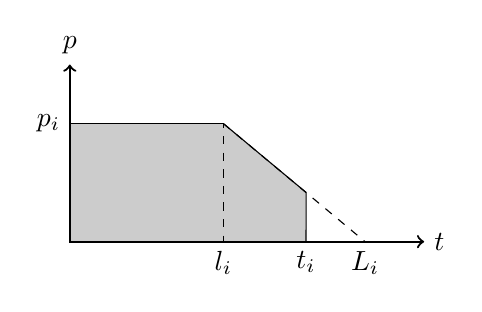
\begin{tikzpicture}[scale=1.5]
\centering
    % Draw axes
    \coordinate (a_1) at (0,1);
    \coordinate (a_2) at (1.3,1);  
    \draw [<->,thick] (0,1.5) node (yaxis) [above] {$p$}
        |- (3,0) node (xaxis) [right] {$t$};
    % Draw two intersecting lines
    
    \draw[dashed] (1.3,1) coordinate (b_1) -- (2.5,0) coordinate (b_2)node[below] {$L_{i}$};
    \draw[opacity=0] (2,0) coordinate (c_1)--(2,1.5) coordinate (c_2);
    % Calculate the intersection of the lines a_1 -- a_2 and b_1 -- b_2
    % and store the coordinate in c.
    \coordinate (c) at (intersection of a_1--a_2 and b_1--b_2);
	\coordinate (d) at (intersection of c_1--c_2 and b_1--b_2);
	\draw (2,0)node [below] {$t_{i}$} -- (d) ;
	\draw (d) -- (b_1) ;
	\fill[opacity=.2] (0,0) -- (a_1) -- (a_2) -- (d) -- (2,0) -- cycle;
	\draw (a_1) -- (a_2);
    % Draw lines indicating intersection with y and x axis. Here we use
    % the perpendicular coordinate system
    \draw[dashed] (yaxis |- c) node[left] {$p_{i}$}
        -| (xaxis -| c) node[below] {$l_{i}$};
    % Draw a dot to indicate intersection point
    %\fill[black] (c) circle (2pt);
\end{tikzpicture}
\caption{Visualized profit function}
\label{fig:graphPF}
\end{figure}

 As shown in Figure \ref{fig:graphPF}, the marginal profit is constant until the minimum service time $l_{i}$ is reached. After this point in time, the marginal profit is decreasing linearly until the maximum service time $L_{i}$ is reached after which the marginal profit is 0. 

\begin{align}
&f(t_{i}) = l_{i}p_{i} + 0.5p_{i}(t_{i}-l_{i}) + \dfrac{p_{i}(t_{i}-l_{i})^{2}}{2(L_{i}-l_{i})} 
\end{align}

The profit function was geometrically derived from the drawn profit function, since the area of the rectangle left of $l_{i}$ was added to the area of the trapezoid between $t_{i}$ and $l_{i}$. Inserting the respective edge lengths in the rectangular as well as the trapezoid area formula is delivering the profit function (17). \\  
The result of the dynamic programming approach is an optimal state for each stage and an optimal decision going from one stage to the next stage. This translates into an optimal starting time $s_{i}$ and an optimal service time $t_{i}$ for each location $i$ as well as an overall objective value which is send back to the HSSA heuristic.

\section{Experimental results}
To test the HSSA heuristic, the modified Solomon instances from Vansteenwegen \cite{Vansteenwegen:2009ils} were used. Due to time limitations, the main tests were conducted using only the first instance of the set, $r101$. All of the Solomon instances contain 100 nodes in addition to the depot and time windows are narrow in that way, that only a small subset of all locations can be visited in one tour. As mentioned previously, the travel time is not included in these instances. The euclidean distances between two nodes, rounded down to the next integer was computed instead. Since Vansteenwegen \cite{Vansteenwegen:2009ils} modified the Solomon instances to accommodate the requirements of the TOPTW, information about the minimum and maximum service time is not given. The setting from Rodriguez and Schmid \cite{Rodriguez:2013}, which chose a minimum service time $l_{i}$ of 5 and a maximum service time $L_{i}$ of 15 for all vertices, was adapted in this experiment. Although the profit stated in the instances of Vansteenwegen \cite{Vansteenwegen:2009ils} were representing the singular collected profit of a location, it was redefined for this experiment to be the base profit $p_{i}$. \\
Since the computational time to solve a TOPTWSTDP with 100 nodes is tremendously big, the idea of partitioning of Rodriguez and Schmid \cite{Rodriguez:2013} was inherited.  

{\renewcommand{\arraystretch}{1.2}
\begin{table}[htbp]
\caption{Partitioning of Solomon instance with 100 locations}
\centering
\begin{tabularx}{\linewidth}{X l l}
\hline 
No. of instances & No. of locations & Instance name\\
\hline
10& 10& 10-1...10-10\\
5& 20& 20-1...20-5\\
3& 30& 30-1...30-3\\
2& 50& 50-1...50-2\\
1& 100& 100-1\\
\hline
\end{tabularx}
\label{tab:r101split}
\end{table} 
Every instance of 100 locations was broken apart into smaller instances of 10, 20, 30, 50 and 100 locations resulting into 21 instances derived from one Solomon instance, illustrated in Table \ref{tab:r101split}.\\
The experiment is divided into two phases: In the first phase, preliminary parameter testing is conducted to determine the best parameters for the HSSA heuristic. In the second phase, the HSSA heuristic is tested on multiple instances using the parameter setting explored in phase one.

\subsection{Preliminary parameter testing}
There are certain parameters, which can be modified to influence the behavior of the hybrid selective simulated annealing heuristic. The first parameter is the initial temperature $T_{0}$, which influences the probability with which a worse solution is still accepted as well as $\alpha$, which is controlling, how fast the the temperature is decreasing after the local search procedure. The determination, how often the local search procedure is applied is dependent on the iteration interval $I_{iter}$. $I_{iter}$ itself is the product of $(n+m-1)Iter_{B}$, whereas $n$ is the number of locations in the instance and m the number of paths. $Iter_{B}$ has to be predefined, which makes the parameter adjustable. Depending on the version of the HSSA heuristic, $T_{max}$ is determining the duration of the heuristic for the fast HSSA version and $N_{non-improving}$ is the termination criteria for the slow HSSA version. These parameters are identical to the simulated annealing heuristic of Lin and Yu \cite{Lin:2012sa}. The only additional parameter added to the heuristic is the iteration interval $S_{iter}$, which is fixing the number of local search moves until a swap of selected and stocked nodes is performed. For all parameters except $S_{iter}$ and $Iter_{B}$, optimal values were inherited from the computational results of Lin and Yu \cite{Lin:2012sa}. Therefore, for the slow hybrid selective simulated annealing (SHSSA) the optimal values are: $T_{0}=0.3$, $\alpha = 0.99$ and $N_{non-improving}=30$.  For the fast hybrid selective simulated annealing (FHSSA) the optimal values are: $T_{0}=0.1$ and $\alpha = 0.999$. 
To evaluate, which value is the best for $Iter_{B}$ and $S_{iter}$, the partitioned Solomon instance r101 was used. Thereby only the first two instances for each instance size were used due to computational time complexity. Both variants of the HSSA, the SHSSA and the FHSSA, were applied three times to each instance. The maximum running time for the fast HSSA heuristic was fixed to $T_{max}=nm$. To minimize randomness, the average computational time and solution of these three runs was taken into consideration. The computation was performed on a cluster with 8 computing nodes, each with 2 Intel Xeon E5-2687W Processors at 3.1GHz and 256 GB of RAM. This scenario was tested for vehicles sizes $m=1$, $m=2$, $m=3$ and $m=4$. In sum, every variant of the HSSA was running 108 times, thus creating a significant benchmark result to compare different settings of $Iter_{B}$ and $S_{iter}$. Experiments with alternating values of $Iter_{B}$ and $S_{iter}$ were conducted, which are visualized in tables \ref{tab:pt100_5}-\ref{tab:pt300_20}.\\
%% $Iter_{B}=100,S_{iter}=5$; $Iter_{B}=100,S_{iter}=10$; $Iter_{B}=100,S_{iter}=20$; $Iter_{B}=200,S_{iter}=5$; $Iter_{B}=200,S_{iter}=10$; $Iter_{B}=200,S_{iter}=20$; $Iter_{B}=300,S_{iter}=5$; $Iter_{B}=300,S_{iter}=10$ and $Iter_{B}=300,S_{iter}=20$

\begin{table}[htbp]
\centering
\caption{Average results for Solomon instance $r101$}
\begin{tabularx}{\linewidth}{X l l l l l l}
\hline 
&&\multicolumn{2}{l}{FHSSA}&& \multicolumn{2}{l}{SHSSA}\\
\cline{3-4}\cline{6-7}
$Iter_{B}$ & $S_{iter}$ & $F_{avg}$ & $T_{avg}(S)$ && $F_{avg}$ & $T_{avg}(S)$\\
\hline
100&5&3144.20&88.89&&3139.36&96.59\\
\textbf{100}&\textbf{10}&\textbf{3163.77}&\textbf{88.89}&&\textbf{3167.91}&\textbf{181.57}\\
100&20&3128.73&88.89&&3186.15&412.79\\
200&5&3127.46&88.89&&3138.66&124.90\\
200&10&3133.03&88.89&&3186.60&305.91\\
200&20&3108.80&88.89&&3194.71&598.25\\
300&5&3121.17&88.89&&3156.93&196.55\\
300&10&3129.97&88.89&&3179.62&350.19\\
300&20&3102.35&88.89&&3191.93&709.60\\
\hline
Max&&3163.77&88.89&&3194.71&709.60\\
Min&&3102.35&88.89&&3139.36&96.59\\
\hline
\end{tabularx}
\label{tab:ptOverall}
\end{table} 

The results of the preliminary test, illustrated in table \ref{tab:ptOverall}, are indicating, that the combination $Iter_{B}=100,S_{iter}=10$  is delivering the best results with respect to the total average solution and computing time. Although several parameter combinations yield better results for the slow HSSA heuristic, those combinations need significantly longer in comparison to the chosen combination. 

{\renewcommand{\arraystretch}{1.2}
\begin{table}[htbp]
\centering
\caption{Results for $Iter_{B}=100$ and $S_{iter}=5$}
\centering
\begin{tabular}{l l l l l l l}
\hline 
&&\multicolumn{2}{l}{FHSSA}&& \multicolumn{2}{l}{SHSSA}\\
\cline{3-4}\cline{6-7}
Instance & m & $F$ & $T(S)$ && $F$ & $T(S)$\\
\hline
r101-10-1&1&950.00&10.00&&950.00&5.58\\
r101-10-2&1&930.00&10.00&&930.00&2.45\\
r101-20-1&1&1130.00&20.00&&1130.00&8.26\\
r101-20-2&1&1515.00&20.00&&1515.00&6.75\\
r101-30-1&1&1416.00&30.02&&1416.00&20.40\\
r101-30-2&1&1736.60&30.00&&1736.60&16.56\\
r101-50-1&1&1806.80&50.00&&1806.80&34.65\\
r101-50-2&1&2390.10&50.00&&2392.75&40.09\\
r101-100-1&1&2600.05&100.00&&2654.00&194.91\\
r101-10-1&2&1505.00&20.00&&1505.00&12.17\\
r101-10-2&2&1451.40&20.00&&1451.40&5.12\\
r101-20-1&2&2025.80&40.00&&2016.20&21.46\\
r101-20-2&2&2660.00&40.00&&2660.00&17.55\\
r101-30-1&2&2519.00&60.00&&2511.00&65.81\\
r101-30-2&2&3133.93&60.00&&3149.35&49.98\\
r101-50-1&2&3576.80&100.00&&3576.80&79.58\\
r101-50-2&2&4005.77&100.00&&4014.65&143.78\\
r101-100-1&2&4570.03&200.00&&4589.35&510.33\\
r101-10-1&3&1730.65&30.00&&1726.58&15.78\\
r101-10-2&3&1766.40&30.00&&1756.40&9.09\\
r101-20-1&3&2807.92&60.00&&2833.72&40.76\\
r101-20-2&3&3416.95&60.00&&3287.97&31.81\\
r101-30-1&3&3534.00&90.00&&3521.73&80.83\\
r101-30-2&3&4150.28&90.00&&4055.72&54.67\\
r101-50-1&3&4755.27&150.0&&4770.78&167.31\\
r101-50-2&3&5231.27&150.00&&5336.50&136.10\\
r101-100-1&3&6156.63&300.0&&6299.15&463.37\\
r101-10-1&4&1815.00&40.00&&1822.27&19.76\\
r101-10-2&4&1946.40&40.00&&1946.40&12.06\\
r101-20-1&4&3251.33&80.00&&3263.80&61.74\\
r101-20-2&4&3818.33&80.00&&3612.27&34.21\\
r101-30-1&4&4203.60&120.00&&4228.67&92.88\\
r101-30-2&4&4900.22&120.00&&4762.05&79.75\\
r101-50-1&4&5843.07&200.00&&5885.20&183.31\\
r101-50-2&4&6397.02&200.00&&6268.40&191.83\\
r101-100-1&4&7544.57&401.00&&7634.32&566.51\\
\hline
Average&&3144.20&88.89&&3139.36&96.59\\
\hline
\end{tabular}
\label{tab:pt100_5}
\end{table}

{\renewcommand{\arraystretch}{1.2}
\begin{table}[htbp]
\centering
\caption{Results for $Iter_{B}=100$ and $S_{iter}=10$}
\centering
\begin{tabular}{l l l l l l l}
\hline 
&&\multicolumn{2}{l}{FHSSA}&& \multicolumn{2}{l}{SHSSA}\\
\cline{3-4}\cline{6-7}
Instance & m & $F$ & $T(S)$ && $F$ & $T(S)$\\
\hline
r101-10-1&1&950.00&10.00&&950.00&8.17\\
r101-10-2&1&930.00&10.00&&930.00&3.68\\
r101-20-1&1&1130.00&20.00&&1130.00&12.83\\
r101-20-2&1&1515.00&20.00&&1515.00&13.84\\
r101-30-1&1&1416.00&30.00&&1416.00&44.17\\
r101-30-2&1&1736.60&30.00&&1736.60&30.06\\
r101-50-1&1&1806.80&50.00&&1806.80&73.28\\
r101-50-2&1&2408.17&50.00&&2405.68&71.53\\
r101-100-1&1&2583.77&100.00&&2644.85&354.63\\
r101-10-1&2&1505.00&20.00&&1505.00&16.24\\
r101-10-2&2&1451.40&20.00&&1451.40&8.14\\
r101-20-1&2&2035.40&40.00&&2025.80&37.93\\
r101-20-2&2&2660.00&40.00&&2660.00&24.20\\
r101-30-1&2&2491.00&60.00&&2519.00&76.26\\
r101-30-2&2&3132.08&60.00&&3124.08&98.69\\
r101-50-1&2&3576.80&100.00&&3576.80&206.42\\
r101-50-2&2&3992.48&100.00&&4035.30&253.20\\
r101-100-1&2&4607.33&200.00&&4607.13&554.83\\
r101-10-1&3&1721.37&30.00&&1731.38&28.32\\
r101-10-2&3&1766.40&30.00&&1756.40&16.62\\
r101-20-1&3&2813.30&60.00&&2811.25&58.27\\
r101-20-2&3&3269.58&60.00&&3315.90&59.01\\
r101-30-1&3&3495.80&90.00&&3573.60&130.86\\
r101-30-2&3&4171.88&90.00&&4089.85&109.36\\
r101-50-1&3&4874.72&150.00&&4789.43&318.06\\
r101-50-2&3&5280.15&150.00&&5362.15&391.86\\
r101-100-1&3&6324.00&300.00&&6454.27&1021.75\\
r101-10-1&4&1815.00&40.00&&1829.53&26.69\\
r101-10-2&4&1946.40&40.00&&1946.40&23.56\\
r101-20-1&4&3230.00&80.00&&3241.23&89.73\\
r101-20-2&4&3866.32&80.00&&3636.67&72.21\\
r101-30-1&4&4262.53&120.00&&4267.00&206.39\\
r101-30-2&4&4790.90&120.00&&4741.97&174.92\\
r101-50-1&4&5975.78&200.00&&5960.38&441.20\\
r101-50-2&4&6365.80&200.00&&6492.50&443.28\\
r101-100-1&4&7998.03&400.00&&8005.23&1036.53\\
\hline
Average&&3163.77&88.89&&3167.91&181.57\\
\hline
\end{tabular}
\label{tab:pt100_10}
\end{table}

{\renewcommand{\arraystretch}{1.2}
\begin{table}[htbp]
\centering
\caption{Results for $Iter_{B}=100$ and $S_{iter}=20$}
\centering
\begin{tabular}{l l l l l l l}
\hline 
&&\multicolumn{2}{l}{FHSSA}&& \multicolumn{2}{l}{SHSSA}\\
\cline{3-4}\cline{6-7}
Instance & m & $F$ & $T(S)$ && $F$ & $T(S)$\\
\hline
r101-10-1&1&950.00&10.00&&950.00&18.14\\
r101-10-2&1&930.00&10.00&&930.00&9.27\\
r101-20-1&1&1130.00&20.00&&1130.00&25.88\\
r101-20-2&1&1515.00&20.00&&1515.00&23.48\\
r101-30-1&1&1416.00&30.00&&1416.00&82.45\\
r101-30-2&1&1736.60&30.00&&1736.60&61.99\\
r101-50-1&1&1806.80&50.00&&1806.80&134.32\\
r101-50-2&1&2374.68&50.00&&2418.75&194.01\\
r101-100-1&1&2611.50&100.00&&2677.50&1064.74\\
r101-10-1&2&1504.80&20.00&&1505.00&29.79\\
r101-10-2&2&1451.40&20.00&&1451.40&15.73\\
r101-20-1&2&2011.67&40.00&&2030.00&86.37\\
r101-20-2&2&2633.33&40.00&&2660.00&58.57\\
r101-30-1&2&2489.00&60.00&&2526.00&166.67\\
r101-30-2&2&3101.25&60.00&&3118.52&126.17\\
r101-50-1&2&3467.00&100.00&&3551.20&370.52\\
r101-50-2&2&3911.92&100.00&&3984.85&375.94\\
r101-100-1&2&4513.73&200.00&&4690.28&1284.22\\
r101-10-1&3&1719.32&30.00&&1729.33&42.38\\
r101-10-2&3&1766.40&30.00&&1736.40&24.01\\
r101-20-1&3&2797.43&60.00&&2780.38&84.44\\
r101-20-2&3&3365.60&60.00&&3365.00&66.70\\
r101-30-1&3&3432.73&90.00&&3564.00&293.75\\
r101-30-2&3&4032.75&90.00&&4114.33&246.15\\
r101-50-1&3&4724.95&150.00&&4863.77&540.88\\
r101-50-2&3&5257.27&150.00&&5317.62&703.25\\
r101-100-1&3&6222.03&300.00&&6492.78&3073.87\\
r101-10-1&4&1815.00&40.00&&1815.00&63.12\\
r101-10-2&4&1946.40&40.00&&1946.40&31.48\\
r101-20-1&4&3253.80&80.00&&3256.00&129.74\\
r101-20-2&4&3621.67&80.00&&3747.27&140.59\\
r101-30-1&4&4168.87&120.00&&4242.87&245.54\\
r101-30-2&4&4731.12&120.00&&4818.70&314.20\\
r101-50-1&4&5907.57&200.00&&6032.53&1197.43\\
r101-50-2&4&6228.48&200.00&&6540.32&925.46\\
r101-100-1&4&8088.05&400.00&&8240.95&2609.02\\
\hline
Average&&3128.73&88.89&&3186.15&412.79\\
\hline
\end{tabular}
\label{tab:pt100_20}
\end{table}

{\renewcommand{\arraystretch}{1.2}
\begin{table}[htbp]
\centering
\caption{Results for $Iter_{B}=200$ and $S_{iter}=5$}
\centering
\begin{tabular}{l l l l l l l}
\hline 
&&\multicolumn{2}{l}{FHSSA}&& \multicolumn{2}{l}{SHSSA}\\
\cline{3-4}\cline{6-7}
Instance & m & $F$ & $T(S)$ && $F$ & $T(S)$\\
\hline
r101-10-1&1&950.00&10.00&&950.00&8.37\\
r101-10-2&1&930.00&10.00&&930.00&4.04\\
r101-20-1&1&1130.00&20.00&&1130.00&13.44\\
r101-20-2&1&1515.00&20.00&&1515.00&12.24\\
r101-30-1&1&1416.00&30.00&&1416.00&35.50\\
r101-30-2&1&1736.60&30.00&&1736.60&28.83\\
r101-50-1&1&1806.80&50.00&&1806.80&53.75\\
r101-50-2&1&2392.75&50.00&&2418.75&98.30\\
r101-100-1&1&2636.90&100.00&&2640.50&264.73\\
r101-10-1&2&1505.00&20.00&&1505.00&24.65\\
r101-10-2&2&1451.40&20.00&&1451.40&9.44\\
r101-20-1&2&2025.80&40.00&&2035.40&39.23\\
r101-20-2&2&2660.00&40.00&&2660.00&32.20\\
r101-30-1&2&2495.60&60.00&&2486.00&64.51\\
r101-30-2&2&3116.67&60.00&&3108.67&55.06\\
r101-50-1&2&3576.80&100.00&&3524.53&115.93\\
r101-50-2&2&3974.48&100.00&&4014.53&153.08\\
r101-100-1&2&4421.30&200.00&&4548.07&439.17\\
r101-10-1&3&1731.10&30.00&&1719.85&19.74\\
r101-10-2&3&1766.40&30.00&&1766.40&13.99\\
r101-20-1&3&2798.30&60.00&&2800.77&60.46\\
r101-20-2&3&3390.28&60.00&&3346.30&43.37\\
r101-30-1&3&3495.00&90.00&&3568.60&133.45\\
r101-30-2&3&4097.50&90.00&&4185.70&108.80\\
r101-50-1&3&4735.27&150.00&&4838.17&208.44\\
r101-50-2&3&5224.07&150.00&&5238.05&318.64\\
r101-100-1&3&6084.28&300.00&&6212.87&680.12\\
r101-10-1&4&1836.80&40.00&&1822.27&29.78\\
r101-10-2&4&1946.40&40.00&&1946.40&26.62\\
r101-20-1&4&3292.93&80.00&&3180.52&60.60\\
r101-20-2&4&3685.00&80.00&&3740.00&60.58\\
r101-30-1&4&4288.67&120.00&&4223.67&105.42\\
r101-30-2&4&4750.75&120.00&&4808.00&81.97\\
r101-50-1&4&5770.97&200.00&&5816.37&290.40\\
r101-50-2&4&6419.38&200.00&&6341.90&190.28\\
r101-100-1&4&7534.22&400.00&&7558.80&611.31\\
\hline
Average&&3127.46&88.89&&3138.66&124.90\\
\hline
\end{tabular}
\label{tab:pt200_5}
\end{table}

{\renewcommand{\arraystretch}{1.2}
\begin{table}[htbp]
\centering
\caption{Results for $Iter_{B}=200$ and $S_{iter}=10$}
\centering
\begin{tabular}{l l l l l l l}
\hline 
&&\multicolumn{2}{l}{FHSSA}&& \multicolumn{2}{l}{SHSSA}\\
\cline{3-4}\cline{6-7}
Instance & m & $F$ & $T(S)$ && $F$ & $T(S)$\\
\hline
r101-10-1&1&950.00&10.00&&950.00&16.82\\
r101-10-2&1&930.00&10.00&&930.00&8.41\\
r101-20-1&1&1130.00&20.00&&1130.00&27.34\\
r101-20-2&1&1515.00&20.00&&1515.00&25.06\\
r101-30-1&1&1416.00&30.00&&1416.00&61.51\\
r101-30-2&1&1736.60&30.00&&1736.60&55.18\\
r101-50-1&1&1806.80&50.00&&1806.80&103.43\\
r101-50-2&1&2360.22&50.00&&2397.50&140.26\\
r101-100-1&1&2670.70&100.00&&2626.35&478.43\\
r101-10-1&2&1505.00&20.00&&1505.00&32.34\\
r101-10-2&2&1451.40&20.00&&1451.40&17.87\\
r101-20-1&2&2035.40&40.00&&2010.80&77.24\\
r101-20-2&2&2633.33&40.00&&2633.33&48.03\\
r101-30-1&2&2521.00&60.00&&2549.00&144.62\\
r101-30-2&2&3116.67&60.00&&3118.52&123.68\\
r101-50-1&2&3551.20&100.00&&3576.80&249.89\\
r101-50-2&2&4022.98&100.00&&4065.35&363.63\\
r101-100-1&2&4604.78&200.00&&4685.87&1183.28\\
r101-10-1&3&1726.58&30.00&&1719.85&42.26\\
r101-10-2&3&1766.40&30.00&&1766.40&35.96\\
r101-20-1&3&2788.78&60.00&&2815.77&105.80\\
r101-20-2&3&3297.32&60.00&&3394.63&81.55\\
r101-30-1&3&3508.80&90.00&&3541.00&152.96\\
r101-30-2&3&4034.88&90.00&&4223.65&315.65\\
r101-50-1&3&4745.85&150.00&&4902.65&635.41\\
r101-50-2&3&5261.72&150.00&&5363.15&510.18\\
r101-100-1&3&6314.50&300.00&&6505.40&1980.08\\
r101-10-1&4&1822.27&40.00&&1797.27&50.92\\
r101-10-2&4&1946.40&40.00&&1946.40&41.39\\
r101-20-1&4&3198.42&80.00&&3316.33&174.29\\
r101-20-2&4&3705.22&80.00&&3642.32&114.12\\
r101-30-1&4&4168.60&120.00&&4310.40&320.23\\
r101-30-2&4&4684.08&120.00&&4813.12&242.73\\
r101-50-1&4&5856.57&200.00&&5941.15&588.30\\
r101-50-2&4&6236.97&200.00&&6572.22&681.16\\
r101-100-1&4&7768.57&400.00&&8041.55&1782.72\\
\hline
Average&&3133.03&88.89&&3186.60&305.91\\
\hline
\end{tabular}
\label{tab:pt200_10}
\end{table}

{\renewcommand{\arraystretch}{1.2}
\begin{table}[htbp]
\centering
\caption{Results for $Iter_{B}=200$ and $S_{iter}=20$}
\centering
\begin{tabular}{l l l l l l l}
\hline 
&&\multicolumn{2}{l}{FHSSA}&& \multicolumn{2}{l}{SHSSA}\\
\cline{3-4}\cline{6-7}
Instance & m & $F$ & $T(S)$ && $F$ & $T(S)$\\
\hline
r101-10-1&1&950.00&10.00&&950.00&33.49\\
r101-10-2&1&930.00&10.00&&930.00&14.80\\
r101-20-1&1&1130.00&20.00&&1130.00&54.51\\
r101-20-2&1&1515.00&20.00&&1515.00&47.14\\
r101-30-1&1&1416.00&30.03&&1416.00&137.73\\
r101-30-2&1&1736.60&30.00&&1736.60&111.42\\
r101-50-1&1&1806.80&50.00&&1806.80&247.90\\
r101-50-2&1&2303.98&50.05&&2414.70&299.13\\
r101-100-1&1&2595.63&100.09&&2657.20&1165.82\\
r101-10-1&2&1497.32&20.00&&1505.00&66.57\\
r101-10-2&2&1451.40&20.00&&1451.40&32.22\\
r101-20-1&2&2020.40&40.00&&2025.80&121.85\\
r101-20-2&2&2633.33&40.00&&2633.33&144.91\\
r101-30-1&2&2471.07&60.07&&2500.60&285.56\\
r101-30-2&2&3065.90&60.03&&3116.67&240.04\\
r101-50-1&2&3420.00&100.00&&3576.80&567.79\\
r101-50-2&2&3955.73&100.00&&4011.92&449.26\\
r101-100-1&2&4392.40&201.38&&4670.28&2169.39\\
r101-10-1&3&1730.65&30.00&&1730.65&111.10\\
r101-10-2&3&1746.40&30.00&&1766.40&63.29\\
r101-20-1&3&2792.92&60.00&&2822.92&265.11\\
r101-20-2&3&3275.00&60.00&&3342.32&179.32\\
r101-30-1&3&3376.80&90.02&&3537.00&403.22\\
r101-30-2&3&4016.72&90.02&&4116.40&654.96\\
r101-50-1&3&4605.97&150.00&&4871.23&897.79\\
r101-50-2&3&5229.72&150.00&&5384.10&744.64\\
r101-100-1&3&6179.75&300.00&&6492.93&3476.44\\
r101-10-1&4&1814.53&40.00&&1829.53&113.62\\
r101-10-2&4&1916.40&40.00&&1946.40&70.89\\
r101-20-1&4&3190.92&80.00&&3303.05&255.87\\
r101-20-2&4&3738.93&80.00&&3790.00&233.35\\
r101-30-1&4&4168.53&120.00&&4359.00&830.83\\
r101-30-2&4&4759.43&120.01&&4828.78&669.38\\
r101-50-1&4&6018.80&200.00&&6092.62&1397.37\\
r101-50-2&4&6368.20&200.19&&6628.38&1037.44\\
r101-100-1&4&7695.62&401.78&&8119.82&3942.79\\
\hline
Average&&3108.80&88.99&&3194.71&598.25\\
\hline
\end{tabular}
\label{tab:pt200_20}
\end{table}

{\renewcommand{\arraystretch}{1.2}
\begin{table}[htbp]
\centering
\caption{Results for Solomon instances for $Iter_{B}=300$ and $S_{iter}=5$}
\centering
\begin{tabular}{l l l l l l l}
\hline 
&&\multicolumn{2}{l}{FHSSA}&& \multicolumn{2}{l}{SHSSA}\\
\cline{3-4}\cline{6-7}
Instance & m & $F$ & $T(S)$ && $F$ & $T(S)$\\
\hline
r101-10-1&1&950.00&10.00&&950.00&11.27\\
r101-10-2&1&930.00&10.00&&930.00&6.26\\
r101-20-1&1&1130.00&20.00&&1130.00&20.44\\
r101-20-2&1&1515.00&20.00&&1515.00&17.09\\
r101-30-1&1&1416.00&30.00&&1416.00&50.82\\
r101-30-2&1&1736.60&30.00&&1736.60&42.03\\
r101-50-1&1&1806.80&50.00&&1806.80&84.21\\
r101-50-2&1&2388.70&50.00&&2408.17&112.50\\
r101-100-1&1&2630.70&100.00&&2675.70&454.33\\
r101-10-1&2&1505.00&20.00&&1505.00&23.46\\
r101-10-2&2&1451.40&20.00&&1451.40&13.24\\
r101-20-1&2&2035.40&40.00&&2020.40&40.50\\
r101-20-2&2&2633.33&40.00&&2660.00&36.71\\
r101-30-1&2&2556.00&60.00&&2525.60&130.86\\
r101-30-2&2&3108.67&60.00&&3132.08&127.52\\
r101-50-1&2&3479.73&100.00&&3531.73&168.09\\
r101-50-2&2&3952.75&100.00&&4050.05&263.10\\
r101-100-1&2&4427.00&200.00&&4600.88&586.32\\
r101-10-1&3&1720.63&30.00&&1727.05&50.89\\
r101-10-2&3&1766.40&30.00&&1766.40&25.81\\
r101-20-1&3&2799.58&60.00&&2813.30&81.66\\
r101-20-2&3&3357.97&60.00&&3389.63&53.50\\
r101-30-1&3&3539.80&90.00&&3523.60&192.36\\
r101-30-2&3&4081.80&90.00&&4140.08&180.03\\
r101-50-1&3&4785.50&150.00&&4785.80&267.07\\
r101-50-2&3&5152.55&150.00&&5245.85&340.55\\
r101-100-1&3&6107.15&300.00&&6124.83&910.87\\
r101-10-1&4&1829.53&40.00&&1815.00&48.90\\
r101-10-2&4&1946.40&40.00&&1936.40&27.77\\
r101-20-1&4&3254.18&80.00&&3256.33&108.68\\
r101-20-2&4&3700.65&80.00&&3805.65&93.76\\
r101-30-1&4&4230.00&120.00&&4232.00&202.82\\
r101-30-2&4&4689.55&120.00&&4878.73&159.46\\
r101-50-1&4&5803.60&200.00&&5939.95&459.50\\
r101-50-2&4&6305.08&200.00&&6351.77&440.33\\
r101-100-1&4&7638.68&400.00&&7871.82&1243.06\\
\hline
Average&&3121.17&88.89&&3156.93&196.55\\
\hline
\end{tabular}
\label{tab:pt300_5}
\end{table}

{\renewcommand{\arraystretch}{1.2}
\begin{table}[htbp]
\centering
\caption{Results for $Iter_{B}=300$ and $S_{iter}=10$}
\centering
\begin{tabular}{l l l l l l l}
\hline 
&&\multicolumn{2}{l}{FHSSA}&& \multicolumn{2}{l}{SHSSA}\\
\cline{3-4}\cline{6-7}
Instance & m & $F$ & $T(S)$ && $F$ & $T(S)$\\
\hline
r101-10-1&1&950.00&10.00&&950.00&25.33\\
r101-10-2&1&930.00&10.00&&930.00&10.95\\
r101-20-1&1&1130.00&20.00&&1130.00&37.91\\
r101-20-2&1&1515.00&20.00&&1515.00&35.03\\
r101-30-1&1&1416.00&30.00&&1416.00&104.21\\
r101-30-2&1&1736.60&30.00&&1736.60&78.37\\
r101-50-1&1&1806.80&50.00&&1806.80&151.80\\
r101-50-2&1&2296.00&50.00&&2414.70&169.01\\
r101-100-1&1&2621.35&100.00&&2639.85&494.88\\
r101-10-1&2&1505.00&20.00&&1505.00&44.72\\
r101-10-2&2&1451.40&20.00&&1451.40&25.92\\
r101-20-1&2&2010.80&40.00&&2020.40&89.83\\
r101-20-2&2&2660.00&40.00&&2633.33&71.24\\
r101-30-1&2&2493.40&60.00&&2521.00&255.27\\
r101-30-2&2&3091.40&60.00&&3106.22&184.01\\
r101-50-1&2&3434.53&100.00&&3576.80&473.99\\
r101-50-2&2&3914.68&100.00&&4086.02&408.44\\
r101-100-1&2&4547.43&200.00&&4732.30&1366.06\\
r101-10-1&3&1722.07&30.00&&1726.58&62.16\\
r101-10-2&3&1766.40&30.00&&1766.40&45.01\\
r101-20-1&3&2813.30&60.00&&2780.38&137.38\\
r101-20-2&3&3268.93&60.00&&3375.28&171.95\\
r101-30-1&3&3406.27&90.00&&3571.00&405.18\\
r101-30-2&3&4047.15&90.00&&4127.80&296.86\\
r101-50-1&3&4740.55&150.00&&4961.80&657.82\\
r101-50-2&3&5273.58&150.00&&5331.50&635.84\\
r101-100-1&3&6355.93&300.00&&6379.02&1806.81\\
r101-10-1&4&1822.27&40.00&&1815.00&89.32\\
r101-10-2&4&1936.40&40.00&&1936.40&48.99\\
r101-20-1&4&3267.60&80.00&&3261.65&161.42\\
r101-20-2&4&3601.67&80.00&&3688.33&149.34\\
r101-30-1&4&4154.00&120.00&&4235.67&326.69\\
r101-30-2&4&4909.15&120.00&&4892.30&359.38\\
r101-50-1&4&5929.03&200.00&&5941.30&696.17\\
r101-50-2&4&6253.62&200.00&&6451.90&563.56\\
r101-100-1&4&7900.53&400.00&&8052.42&1965.87\\
\hline
Average&&3129.97&88.89&&3179.62&350.19\\
\hline
\end{tabular}
\label{tab:pt300_10}
\end{table}

{\renewcommand{\arraystretch}{1.2}
\begin{table}[htbp]
\centering
\caption{Results for $Iter_{B}=300$ and $S_{iter}=20$}
\centering
\begin{tabular}{l l l l l l l}
\hline 
&&\multicolumn{2}{l}{FHSSA}&& \multicolumn{2}{l}{SHSSA}\\
\cline{3-4}\cline{6-7}
Instance & m & $F$ & $T(S)$ && $F$ & $T(S)$\\
\hline
r101-10-1&1&950.00&10.00&&950.00&46.38\\
r101-10-2&1&930.00&10.00&&930.00&24.17\\
r101-20-1&1&1130.00&20.00&&1130.00&77.46\\
r101-20-2&1&1515.00&20.00&&1515.00&71.89\\
r101-30-1&1&1416.00&30.00&&1416.00&197.87\\
r101-30-2&1&1736.60&30.00&&1736.60&170.23\\
r101-50-1&1&1802.87&50.00&&1806.80&285.98\\
r101-50-2&1&2332.17&50.00&&2418.75&401.29\\
r101-100-1&1&2648.50&100.00&&2647.40&1473.76\\
r101-10-1&2&1505.00&20.00&&1505.00&96.22\\
r101-10-2&2&1451.40&20.00&&1451.40&45.67\\
r101-20-1&2&2020.40&40.00&&2025.80&225.86\\
r101-20-2&2&2630.00&40.00&&2606.67&169.84\\
r101-30-1&2&2488.80&60.00&&2571.00&507.20\\
r101-30-2&2&3066.72&60.00&&3118.52&349.47\\
r101-50-1&2&3446.67&100.00&&3576.80&782.08\\
r101-50-2&2&3841.15&100.00&&4060.88&875.28\\
r101-100-1&2&4450.72&200.00&&4700.90&3613.84\\
r101-10-1&3&1714.80&30.00&&1723.38&162.55\\
r101-10-2&3&1766.40&30.00&&1766.40&74.33\\
r101-20-1&3&2785.77&60.00&&2810.38&285.82\\
r101-20-2&3&3116.80&60.00&&3420.28&327.02\\
r101-30-1&3&3401.60&90.00&&3537.07&614.11\\
r101-30-2&3&4070.73&90.00&&4102.22&617.41\\
r101-50-1&3&4655.60&150.00&&4881.80&1095.31\\
r101-50-2&3&5302.17&150.00&&5355.40&1155.82\\
r101-100-1&3&6317.53&300.00&&6454.57&3331.50\\
r101-10-1&4&1797.27&40.00&&1822.27&192.45\\
r101-10-2&4&1936.40&40.00&&1946.40&101.10\\
r101-20-1&4&3235.13&80.00&&3248.80&400.89\\
r101-20-2&4&3603.33&80.00&&3825.65&290.49\\
r101-30-1&4&4037.00&120.00&&4372.00&677.83\\
r101-30-2&4&4756.18&120.00&&4806.18&665.68\\
r101-50-1&4&5784.10&200.00&&6019.80&1207.71\\
r101-50-2&4&6448.93&200.00&&6470.07&961.17\\
r101-100-1&4&7592.78&400.00&&8179.13&3969.87\\
\hline
Average&&3102.35&88.89&&3191.93&709.60\\
\hline
\end{tabular}
\label{tab:pt300_20}
\end{table}

%{\renewcommand{\arraystretch}{1.2}
%\begin{table}[htbp]
%\centering
%\caption{Results for Solomon instances (m = 1)}
%\centering
%\begin{tabular}{l l l l l l l l l l}
%\hline 
%&&&\multicolumn{3}{l}{FHSSA}&& \multicolumn{3}{l}{SHSSA}\\
%\cline{4-6}\cline{8-10}
%Instance & m & & $F_{best}$ & $F_{average}$ & $T_{average}(S)$ && $F_{best}$ & $F_{average}$ & $T_{average}(S)$)\\
%\hline
%r101-10-1& 1&& 950.00& 930.00& 50.00&&950.00& 930.00& 50.00\\
%\hline
%Average &&&&&&&0.05&&0.03\\
%\hline
%\end{tabular}
%\end{table}

\subsection{Benchmark results}
After the determination of $Iter_{B}$ and $S_{iter}$ in the preliminary test, benchmark runs were conducted. Each of the 21 instances of $r101$ were solved with differing vehicle numbers from $m=1$ to $m=3$. For the one vehicle ($m=1$) scenario, MIP was additionally applied besides the two heuristics to evaluate the optimal solution for the respective instance. The MIP was facilitated using the CPLEX environment (concert technology) within C++. For these instances, the FHSSA and SHSSA stopped after reaching the optimal solution. FHSSA and SHSSA were applied five times per instance, thus generating robust average solutions and computational times.\\ 
The maximum running time for the fast HSSA heuristic was fixed to $T_{max}=nm$. Parameters except $S_{iter}$ and $Iter_{B}$ were, as in the preliminary test, inherited from the computational results of Lin and Yu \cite{Lin:2012sa}. For the slow hybrid selective simulated annealing (SHSSA) the parameters are: $T_{0}=0.3$, $\alpha = 0.99$ and $N_{non-improving}=30$.  For the fast hybrid selective simulated annealing (FHSSA) the parameters are: $T_{0}=0.1$ and $\alpha = 0.999$. The computation was also performed on a cluster with 8 computing nodes, each with 2 Intel Xeon E5-2687W Processors at 3.1GHz and 256 GB of RAM. \\
The results, illustrated in table \ref{tab:bm_1}-\ref{tab:bm_3}, indicate, that both of the HSSA variants are robust. For all instances sizes, the maximum gap to the optimal solution, were measurable, was at most 2\%. Computational times for the FHSSA and the SHSSA were also significantly lower then those of the MIP. \\
Additionally to the benchmark result for Solomon instance r101, further results for other Solomon instances are provided in the appendix.\\ 
 

{\renewcommand{\arraystretch}{1.2}
\begin{table*}[htbp]
\caption{Results for Solomon instances for $m=1$}
\centering
\begin{tabularx}{\linewidth}{m{4.5em} l l l l l l l l l l l l}
\hline
& \multicolumn{2}{l}{MIP}&&\multicolumn{4}{l}{FHSSA}&& \multicolumn{4}{l}{SHSSA}\\
%\cline{2-3}\cline{5-8}\cline{10-13}
\hline
Instance & Solution & T (S) & & $F_{Best}$ & $F_{Average}$  & Gap (\%) & T (S) & & $F_{Best}$ & $F_{Average}$  & Gap (\%) & T (S)\\
\hline
r101-10-1&950.00&4.25&&950.00&950.00&0.00&10.00&&950.00&950.00&0.00& 10.35\\
r101-10-2&930.00&15.49&&930.00&930.00&0.00&0.01&&930.00&930.00&0.00& 0.00\\
r101-10-3&1130.00&7.65&&1130.00&1130.00&0.00&0.29&&1130.00&1130.00& 0.00&0.16\\
r101-10-4&945.00&11.67&&945.00&945.00&0.00&0.00&&945.00&945.00&0.00& 0.02\\
r101-10-5&1551.80&21.85&&1551.80&1551.80&0.00&10.00&&1551.80&1551.80& 0.00&10.15\\
r101-10-6&1315.00&28.53&&1315.00&1315.00&0.00&0.33&&1315.00&1315.00& 0.00&0.56\\
r101-10-7&1050.00&12.82&&1050.00&1050.00&0.00&0.08&&1050.00&1050.00& 0.00&0.13\\
r101-10-8&1174.60&12.11&&1174.60&1174.60&0.00&10.00&&1174.60&1174.60& 0.00&10.07\\
r101-10-9&1148.20&5.14&&1148.20&1148.20&0.00&0.02&&1148.20&1148.20& 0.00&0.08\\
r101-10-10&1645.65&40.70&&1645.65&1631.46&0.01&10.00&&1645.65&1617.27& 0.02&8.14\\
r101-20-1&1130.00&28.00&&1130.00&1130.00&0.00&0.08&&1130.00&1130.00&0.00&0.09\\
r101-20-2&1515.00&20.32&&1515.00&1515.00&0.00&20.00&&1515.00&1515.00&0.00&16.82\\
r101-20-3&1613.40&38.13&&1613.40&1613.40&0.00&0.55&&1613.40&1613.40&0.00&0.85\\
r101-20-4&1665.00&35.30&&1665.00&1665.00&0.00&0.66&&1665.00&1665.00&0.00&0.72\\
r101-20-5&1849.65&275.66&&1849.65&1825.65&0.01&20.00&&1849.65&1825.65&0.01&24.23\\
r101-30-1&1416.00&193.94&&1416.00&1416.00&0.00&30.00&&1416.00&1416.00&0.00&48.02\\
r101-30-2&1736.60&104.82&&1736.60&1736.60&0.00&4.38&&1736.60&1736.60&0.00&4.59\\
r101-30-3&1805.00&68.01&&1805.00&1805.00&0.00&30.00&&1805.00&1805.00&0.00&42.65\\
r101-50-1&1806.80&575.87&&1806.80&1806.80&0.00&50.00&&1806.80&1806.80&0.00&82.31\\
r101-50-2&2418.75&30588.26&&2418.75&2392.66&0.01&38.32&&2418.75&2403.15&0.01&58.83\\
r101-100-1&n/a&n/a&&2677.50&2627.94&n/a&100.00&&2677.50&2667.93&n/a&492.00\\
\hline
Average &&&&&&0.00&&&&&0.00\\
Max &&&&&&0.01&&&&&0.02\\
\hline
\end{tabularx}
\label{tab:bm_1}
\end{table*}

\begin{table*}[htbp]
\caption{Results for Solomon instances for $m=2$}
\centering
\begin{tabularx}{\linewidth}{m{4.5em} l l l l l l l l l l l l}
\hline
& \multicolumn{2}{l}{MIP}&&\multicolumn{4}{l}{FHSSA}&& \multicolumn{4}{l}{SHSSA}\\
%\cline{2-3}\cline{5-8}\cline{10-13}
\hline
Instance & Solution & T (S) & & $F_{Best}$ & $F_{Average}$  & Gap (\%) & T (S) & & $F_{Best}$ & $F_{Average}$  & Gap (\%) & T (S)\\
\hline
r101-10-1&1505.00&1243.69&&1505.00&1505.00&0.00&20.00&&1505.00&1504.88&0.00&22.03\\
r101-10-2&1451.40&52.89&&1451.40&1451.40&0.00&1.08&&1451.40&1451.40&0.00&1.21\\
r101-10-3&1730.00&368.11&&1730.00&1712.00&0.01&11.93&&1730.00&1712.00&0.01&12.01\\
r101-10-4&1680.00&30.55&&1680.00&1680.00&0.00&1.17&&1680.00&1680.00&0.00&0.81\\
r101-10-5&2100.00&76.57&&2100.00&2100.00&0.00&20.00&&2100.00&2100.00&0.00&16.71\\
r101-10-6&1545.00&986.34&&1545.00&1545.00&0.00&2.51&&1545.00&1545.00&0.00&1.18\\
r101-10-7&1800.00&23.22&&1800.00&1800.00&0.00&1.01&&1800.00&1800.00&0.00&0.64\\
r101-10-8&1667.10&1650.78&&1667.10&1667.10&0.00&3.55&&1667.10&1664.78&0.00&5.88\\
r101-10-9&1770.00&82.91&&1770.00&1770.00&0.00&0.25&&1770.00&1770.00&0.00&0.12\\
r101-10-10&1965.00&11180.29&&1965.00&1962.00&0.00&6.82&&1965.00&1956.00&0.00&7.48\\
r101-20-1&n/a &n/a&&2045.00&2021.96&n/a&40.00&&2045.00&2033.48&n/a&49.95\\
r101-20-2&n/a&n/a&&2660.00&2644.00&n/a&40.00&&2660.00&2660.00&n/a&32.05\\
r101-20-3&n/a&n/a&&2886.80&2879.66&n/a&40.00&&2886.80&2862.23&n/a&33.08\\
r101-20-4&n/a&n/a&&2709.90&2709.90&n/a&40.00&&2709.90&2709.90&n/a&33.35\\
r101-20-5&n/a&n/a&&2984.85&2968.98&n/a&40.00&&2998.05&2972.67&n/a&37.58\\
r101-30-1&n/a&n/a&&2496.00&2475.60&n/a&60.00&&2599.80&2516.64&n/a&89.36\\
r101-30-2&n/a&n/a&&3149.35&3109.02&n/a&60.00&&3103.10&3096.08&n/a&83.72\\
r101-30-3&n/a&n/a&&3068.75&3039.71&n/a&60.00&&3124.25&3087.15&n/a&71.65\\
r101-50-1&n/a&n/a&&3576.80&3475.72&n/a&100.00&&3576.80&3498.72&n/a&191.45\\
r101-50-2&n/a&n/a&&4059.75&4016.08&n/a&100.00&&4107.65&4041.96&n/a&205.00\\
r101-100-1&n/a&n/a&&4658.95&4553.48&n/a&200.00&&4735.35&4656.61&n/a&761.59\\
\hline
Average &&&&&&0.00&&&&&0.00\\
Max &&&&&&0.01&&&&&0.01\\
\hline
\end{tabularx}
\label{tab:bm_2}
\end{table*}

\begin{table*}[htbp]
\caption{Results for Solomon instances for $m=3$}
\centering
\begin{tabularx}{\linewidth}{X l l l l l l l l l l l l}
\hline
& \multicolumn{2}{l}{MIP}&&\multicolumn{4}{l}{FHSSA}&& \multicolumn{4}{l}{SHSSA}\\
%\cline{2-3}\cline{5-8}\cline{10-13}
\hline
Instance & Solution & T (S) & & $F_{Best}$ & $F_{Average}$  & Gap (\%) & T (S) & & $F_{Best}$ & $F_{Average}$  & Gap (\%) & T (S)\\
\hline
r101-10-1&n/a&n/a&&1736.60&1723.52&n/a&30.00&&1736.60&1727.46&n/a&33.32\\
r101-10-2&n/a&n/a&&1766.40&1766.40&n/a&30.00&&1766.40&1760.40&n/a&17.47\\
r101-10-3&n/a&n/a&&2055.00&2055.00&n/a&30.00&&2055.00&2046.00&n/a&21.11\\
r101-10-4&n/a&n/a&&2040.00&2025.00&n/a&30.00&&2040.00&2025.00&n/a&19.71\\
r101-10-5&n/a&n/a&&2355.00&2340.00&n/a&30.00&&2355.00&2295.00&n/a&19.72\\
r101-10-6&n/a&n/a&&1705.00&1701.00&n/a&30.00&&1705.00&1699.00&n/a&19.23\\
r101-10-7&n/a&n/a&&2100.00&2100.00&n/a&30.00&&2100.00&2100.00&n/a&10.56\\
r101-10-8&n/a&n/a&&1895.10&1892.70&n/a&30.00&&1895.10&1892.70&n/a&26.83\\
r101-10-9&n/a&n/a&&2160.00&2160.00&n/a&30.00&&2160.00&2160.00&n/a&15.99\\
r101-10-10&n/a&n/a&&1965.00&1965.00&n/a&30.00&&1965.00&1959.00&n/a&12.45\\
r101-20-1&n/a&n/a&&2820.00&2799.52&n/a&60.00&&2836.15&2796.92&n/a&71.25\\
r101-20-2&n/a&n/a&&3426.95&3317.78&n/a&60.00&&3380.00&3321.76&n/a&81.30\\
r101-20-3&n/a&n/a&&3490.40&3479.40&n/a&60.00&&3499.00&3465.32&n/a&78.81\\
r101-20-4&n/a&n/a&&3418.15&3316.48&n/a&60.00&&3395.75&3289.24&n/a&58.03\\
r101-20-5&n/a&n/a&&3890.50&3841.54&n/a&60.00&&3845.50&3783.58&n/a&37.99\\
r101-30-1&n/a&n/a&&3561.00&3499.08&n/a&90.00&&3553.80&3480.84&n/a&113.70\\
r101-30-2&n/a&n/a&&4208.95&4129.36&n/a&90.00&&4281.85&4152.69&n/a&175.63\\
r101-30-3&n/a&n/a&&4224.85&4144.06&n/a&90.00&&4143.75&4116.43&n/a&185.92\\
r101-50-1&n/a&n/a&&4881.80&4771.08&n/a&150.00&&4961.80&4905.00&n/a&334.04\\
r101-50-2&n/a&n/a&&5383.25&5289.58&n/a&150.00&&5482.85&5382.14&n/a&360.76\\
r101-100-1&n/a &n/a&&6507.05&6372.13&n/a&300.00&&6576.05&6452.01&n/a&1411.22\\
\hline
Average &&&&&&n/a&&&&&n/a\\
Max &&&&&&n/a&&&&&n/a\\
\hline
\end{tabularx}
\label{tab:bm_3}
\end{table*}


%%%\begin{landscape}
%\begin{table}[h]
%\centering
%\begin{tabular}{l l l l l l l l l l l l l l l l l l l}
%\hline
%Instance & MIP & T(S) & & FHSSA & T(S) & & SHSSA & T(S) && Instance & MIP & T(S) & & FHSSA & T(S) & & SHSSA & T(S)\\
%\hline
%T 1 & 0.0003262 & 0.562 \\
%T 2 & 0.0015681 & 0.910 \\
%T 3 & 0.0009271 & 0.296 \\
%\hline
%\end{tabular}
%\caption{Table caption}
%\end{table}
%%%\end{landscape}

\section{Conclusions and further research}
In this paper, the team orienteering problem with time windows and service time dependent profit was introduced. The aim of this problem class is to maximize the total collected profit for a given number of routes and locations. In constrast to the TOPTW, a vehicle visiting one location is not only collecting a one time profit independent of its stay in that location. In the TOPTWSTDP, the vehicle is constantly collecting marginal profit until a maximum service time is reached. In addition, the vehicle also has to stay for a predefined period of time. The marginal profit is increasing after the minimum service time until it equals zero when the vehicle is staying in the respective location until the maximum service time is reached. Due to the variable profit that can be collected at each location, the TOPTWSTDP is, in comparison to the TOPTW, not only a routing problem but also a scheduling problem, since decisions have to be made when a vehicle should arrive at one location and how long it has to stay there. \\
For the TOPTWSTDP, a mathematical model was provided to solve small instances using mixed integer programming. For large instances and vehicle numbers MIP is infeasible due to exponentially increasing computation times. For those scenarios a hybrid selective simulated annealing heuristic was proposed in this paper. The basic idea of altering a given sequence of locations was adopted from Lin and Yu \citep{Lin:2012sa}. An extension of the simulated annealing (SA) heuristic was the assumption, that few locations can be visited during one tour, thus making it inefficient to include all possible locations in the sequence. The HSSA heuristic only selects a subset of possible locations, whereas the selection is altered periodically throughout the algorithm. Another extension of the SA heuristic was the addition of a dynamic programming (DP) approach, which became necessary due to the new service time dependent profit aspect of the TOPTWSTDP. The objective value was now evaluated using DP instead of adding up one time profits of visited locations. \\
Further on, the paper determined optimal values of $S_{iter}$, an additional parameter used in comparison to the SA heuristic of Lin and Yu \cite{Lin:2012sa}, for both HSSA variants. \\
Since the TOPTWSTDP is a new extension of the TOPTW, no benchmark solutions of other heuristics exist. The aim of the paper therefore was to provide heuristical benchmark solutions and exact solutions for small instances and vehicle numbers. \\
Although the parameter settings of Lin and Yu \cite{Lin:2012sa} were optimal for the SA heuristic they were proposing, it stands to question, whether this assumption still holds for the HSSA heuristic. Future research may try to evaluate the best parameter settings for the HSSA, thus rejecting or accepting the optimal values of Lin and Yu     \cite{Lin:2012sa}. An excellent approach to determine the best combination of these parameters would be the application of an F-Race, proposed by Birattari et al. \cite{Birattari:2010frace}, which iteratively is evaluating different parameter settings and ultimately is delivering the best possible parameter combination. \\
Further research may also try to find other meta-heuristics to tackle the TOPTWSTDP, since the HSSA heuristic, although it is delivering high quality results, requires non neglectable amount of computing time, which makes it impossible to apply the heuristic in situations where fast results matter. 

%\begin{itemize}
%\item Bullet point one
%\item Bullet point two
%\end{itemize}
%
%\begin{enumerate}
%\item Numbered list item one
%\item Numbered list item two
%\end{enumerate}

%% The Appendices part is started with the command \appendix;
%% appendix sections are then done as normal sections
%% \appendix

%% \section{}
%% \label{}

%% References
%%
%% Following citation commands can be used in the body text:
%% Usage of \cite is as follows:
%%   \cite{key}          ==>>  [#]
%%   \cite[chap. 2]{key} ==>>  [#, chap. 2]
%%   \citet{key}         ==>>  Author [#]

%% References with bibTeX database:

\section*{References}
\bibliography{literature}
\bibliographystyle{abbrv}

\onecolumn

\section*{Appendix}
\renewcommand{\thesubsection}{\Alph{subsection}}
\subsection{Benchmark Results for $m=1$}
\begin{longtable}{l l l l l l l l l l l l l}
%\caption{Benchmark Results for Solomon instances $r101, r102, r103$ and $r104$ ($n=10$, $m=1$)}
%\label{tab:bm_A1}
%\centering
%\begin{tabularx}{\linewidth}{m{4.5em} l l l l l l l l l l l l}
\hline
& \multicolumn{2}{l}{MIP}&&\multicolumn{4}{l}{FHSSA}&& \multicolumn{4}{l}{SHSSA}\\
%\cline{2-3}\cline{5-8}\cline{10-13}
\hline
Instance & Solution & T (S) & & $F_{Best}$ & $F_{Average}$  & Gap (\%) & T (S) & & $F_{Best}$ & $F_{Average}$  & Gap (\%) & T (S)\\
\hline
\endhead
r102-10-1& n/a& n/a&&1245.50& 1245.50& n/a& 10.00&&1245.50& 1245.50& n/a& 60.55\\
r102-10-2& n/a& n/a&&1215.00& 1215.00& n/a& 10.00&&1215.00& 1215.00& n/a& 26.01\\
r102-10-3& n/a& n/a&&1295.00& 1295.00& n/a& 10.00&&1295.00& 1295.00& n/a& 44.66\\
r102-10-4& n/a& n/a&&1425.00& 1425.00& n/a& 10.00&&1425.00& 1425.00& n/a& 40.76\\
r102-10-5& n/a& n/a&&1746.80& 1746.80& n/a& 10.00&&1746.80& 1746.80& n/a& 47.60\\
r102-10-6& n/a& n/a&&1315.00& 1315.00& n/a& 10.00&&1315.00& 1315.00& n/a& 18.70\\
r102-10-7& n/a& n/a&&1050.00& 1050.00& n/a& 10.00&&1050.00& 1050.00& n/a& 3.35\\
r102-10-8& n/a& n/a&&1395.00& 1395.00& n/a& 10.00&&1395.00& 1395.00& n/a& 23.37\\
r102-10-9& n/a& n/a&&1770.00& 1770.00& n/a& 10.00&&1770.00& 1770.00& n/a& 37.24\\
r102-10-10& n/a& n/a&&1763.10& 1740.66& n/a& 10.00&&1763.10& 1760.10& n/a& 48.63\\
r103-10-1& n/a& n/a&&1245.50& 1245.50& n/a& 10.00&&1245.50& 1245.50& n/a& 65.18\\
r103-10-2& n/a& n/a&&1601.40& 1601.40& n/a& 10.00&&1601.40& 1601.40& n/a& 79.45\\
r103-10-3& n/a& n/a&&1545.00& 1518.00& n/a& 10.00&&1545.00& 1545.00& n/a& 142.93\\
r103-10-4& n/a& n/a&&1425.00& 1425.00& n/a& 10.00&&1425.00& 1425.00& n/a& 96.20\\
r103-10-5& n/a& n/a&&1845.00& 1842.00& n/a& 10.00&&1845.00& 1845.00& n/a& 117.67\\
r103-10-6& n/a& n/a&&1455.00& 1452.10& n/a& 10.00&&1455.00& 1455.00& n/a& 63.51\\
r103-10-7& n/a& n/a&&1130.60& 1130.60& n/a& 10.00&&1130.60& 1130.60& n/a& 14.72\\
r103-10-8& n/a& n/a&&1480.80& 1480.12& n/a& 10.00&&1480.80& 1480.80& n/a& 42.33\\
r103-10-9& n/a& n/a&&2252.80& 2234.93& n/a& 10.00&&2252.80& 2252.80& n/a& 210.77\\
r103-10-10& n/a& n/a&&1763.10& 1745.10& n/a& 10.00&&1763.10& 1763.10& n/a& 76.92\\
r104-10-1& n/a& n/a&&1291.00& 1276.40& n/a& 10.00&&1291.00& 1291.00& n/a& 107.05\\
r104-10-2& n/a& n/a&&1601.40& 1601.40& n/a& 10.00&&1601.40& 1601.40& n/a& 85.39\\
r104-10-3& n/a& n/a&&1920.00& 1725.00& n/a& 10.00&&1920.00& 1920.00& n/a& 279.38\\
r104-10-4& n/a& n/a&&1652.55& 1593.63& n/a& 10.00&&1652.55& 1652.55& n/a& 188.74\\
r104-10-5& n/a& n/a&&1905.00& 1881.00& n/a& 10.00&&1905.00& 1905.00& n/a& 170.01\\
r104-10-6& n/a& n/a&&1455.00& 1446.30& n/a& 10.00&&1455.00& 1455.00& n/a& 75.79\\
r104-10-7& n/a& n/a&&1675.00& 1665.00& n/a& 10.00&&1675.00& 1675.00& n/a& 132.29\\
r104-10-8& n/a& n/a&&1510.20& 1502.36& n/a& 10.00&&1510.20& 1507.04& n/a& 81.17\\
r104-10-9& n/a& n/a&&2253.00& 2241.31& n/a& 10.00&&2253.00& 2253.00& n/a& 252.84\\
r104-10-10& n/a& n/a&&1959.80& 1843.96& n/a& 10.00&&1965.00& 1965.00& n/a& 200.27\\
r105-10-1& n/a& n/a&&1110.00& 1110.00& n/a& 10.00&&1110.00& 1110.00& n/a& 17.98\\
r105-10-2& n/a& n/a&&1122.40& 1122.40& n/a& 10.00&&1122.40& 1122.40& n/a& 14.86\\
r105-10-3& n/a& n/a&&1347.60& 1347.08& n/a& 10.00&&1347.60& 1347.60& n/a& 33.95\\
r105-10-4& n/a& n/a&&1125.00& 1125.00& n/a& 10.00&&1125.00& 1125.00& n/a& 15.91\\
r105-10-5& n/a& n/a&&1650.00& 1650.00& n/a& 10.00&&1650.00& 1650.00& n/a& 18.02\\
r105-10-6& n/a& n/a&&1395.00& 1395.00& n/a& 10.00&&1395.00& 1395.00& n/a& 16.96\\
r105-10-7& n/a& n/a&&1220.00& 1220.00& n/a& 10.00&&1220.00& 1220.00& n/a& 15.05\\
r105-10-8& n/a& n/a&&1290.00& 1290.00& n/a& 10.00&&1290.00& 1290.00& n/a& 29.87\\
r105-10-9& n/a& n/a&&1615.20& 1615.20& n/a& 10.00&&1615.20& 1615.20& n/a& 9.53\\
r105-10-10& n/a& n/a&&1950.00& 1857.00& n/a& 10.00&&1950.00& 1944.00& n/a& 46.05\\
r106-10-1& n/a& n/a&&1293.25& 1293.25& n/a& 10.00&&1293.25& 1293.25& n/a& 82.11\\
r106-10-2& n/a& n/a&&1395.00& 1395.00& n/a& 10.00&&1395.00& 1395.00& n/a& 38.22\\
r106-10-3& n/a& n/a&&1495.50& 1462.62& n/a& 10.00&&1495.50& 1487.40& n/a& 119.17\\
r106-10-4& n/a& n/a&&1425.00& 1425.00& n/a& 10.00&&1425.00& 1425.00& n/a& 54.76\\
r106-10-5& n/a& n/a&&1835.55& 1834.44& n/a& 10.00&&1835.55& 1835.55& n/a& 65.71\\
r106-10-6& n/a& n/a&&1395.00& 1395.00& n/a& 10.00&&1395.00& 1395.00& n/a& 40.06\\
r106-10-7& n/a& n/a&&1220.00& 1220.00& n/a& 10.00&&1220.00& 1220.00& n/a& 14.15\\
r106-10-8& n/a& n/a&&1466.15& 1463.04& n/a& 10.00&&1466.15& 1466.15& n/a& 56.08\\
r106-10-9& n/a& n/a&&1931.20& 1931.20& n/a& 10.00&&1931.20& 1931.20& n/a& 68.74\\
r106-10-10& n/a& n/a&&1965.00& 1947.00& n/a& 10.00&&1965.00& 1965.00& n/a& 90.08\\
r107-10-1& n/a& n/a&&1293.25& 1293.25& n/a& 10.00&&1293.25& 1293.25& n/a& 83.42\\
r107-10-2& n/a& n/a&&1601.40& 1601.40& n/a& 10.00&&1601.40& 1601.40& n/a& 91.87\\
r107-10-3& n/a& n/a&&1686.30& 1625.52& n/a& 10.00&&1686.30& 1686.30& n/a& 173.55\\
r107-10-4& n/a& n/a&&1465.00& 1465.00& n/a& 10.00&&1465.00& 1465.00& n/a& 99.18\\
r107-10-5& n/a& n/a&&1830.00& 1830.00& n/a& 10.00&&1845.00& 1845.00& n/a& 124.22\\
r107-10-6& n/a& n/a&&1455.00& 1455.00& n/a& 10.00&&1455.00& 1455.00& n/a& 70.96\\
r107-10-7& n/a& n/a&&1220.00& 1220.00& n/a& 10.00&&1220.00& 1220.00& n/a& 32.49\\
r107-10-8& n/a& n/a&&1601.15& 1554.79& n/a& 10.00&&1601.15& 1601.15& n/a& 64.76\\
r107-10-9& n/a& n/a&&2310.00& 2255.55& n/a& 10.00&&2310.00& 2310.00& n/a& 220.89\\
r107-10-10& n/a& n/a&&1965.00& 1917.00& n/a& 10.00&&1965.00& 1962.00& n/a& 116.83\\
r108-10-1& n/a& n/a&&1293.25& 1283.27& n/a& 10.00&&1321.25& 1321.25& n/a& 114.79\\
r108-10-2& n/a& n/a&&1601.40& 1601.40& n/a& 10.00&&1601.40& 1601.40& n/a& 99.87\\
r108-10-3& n/a& n/a&&1920.00& 1880.84& n/a& 10.00&&1920.00& 1920.00& n/a& 309.17\\
r108-10-4& n/a& n/a&&1652.55& 1636.48& n/a& 10.00&&1652.55& 1652.55& n/a& 189.75\\
r108-10-5& n/a& n/a&&1935.20& 1925.08& n/a& 10.00&&1935.20& 1935.20& n/a& 175.17\\
r108-10-6& n/a& n/a&&1455.00& 1449.00& n/a& 10.00&&1455.00& 1455.00& n/a& 83.03\\
r108-10-7& n/a& n/a&&1725.00& 1685.00& n/a& 10.00&&1725.00& 1725.00& n/a& 155.03\\
r108-10-8& n/a& n/a&&1622.00& 1595.31& n/a& 10.00&&1622.00& 1617.83& n/a& 119.41\\
r108-10-9& n/a& n/a&&2310.00& 2292.75& n/a& 10.00&&2310.00& 2310.00& n/a& 240.06\\
r108-10-10& n/a& n/a&&1965.00& 1935.00& n/a& 10.00&&1965.00& 1962.00& n/a& 330.66\\
r109-10-1& n/a& n/a&&1192.40& 1192.40& n/a& 10.00&&1192.40& 1192.40& n/a& 56.09\\
r109-10-2& n/a& n/a&&1180.20& 1180.20& n/a& 10.00&&1180.20& 1180.20& n/a& 51.79\\
r109-10-3& n/a& n/a&&1605.00& 1605.00& n/a& 10.00&&1631.25& 1610.25& n/a& 75.97\\
r109-10-4& n/a& n/a&&1277.55& 1277.55& n/a& 10.00&&1277.55& 1277.55& n/a& 43.50\\
r109-10-5& n/a& n/a&&1725.60& 1725.60& n/a& 10.00&&1725.60& 1725.60& n/a& 46.12\\
r109-10-6& n/a& n/a&&1419.40& 1412.54& n/a& 10.00&&1419.40& 1419.40& n/a& 97.26\\
r109-10-7& n/a& n/a&&1569.50& 1569.50& n/a& 10.00&&1569.50& 1569.50& n/a& 53.60\\
r109-10-8& n/a& n/a&&1515.00& 1515.00& n/a& 10.00&&1515.00& 1515.00& n/a& 57.83\\
r109-10-9& n/a& n/a&&1805.00& 1805.00& n/a& 10.00&&1805.00& 1805.00& n/a& 34.68\\
r109-10-10& n/a& n/a&&1965.00& 1845.00& n/a& 10.00&&1965.00& 1964.19& n/a& 174.40\\
r110-10-1& n/a& n/a&&1260.00& 1260.00& n/a& 10.00&&1260.00& 1260.00& n/a& 66.32\\
r110-10-2& n/a& n/a&&1335.00& 1335.00& n/a& 10.00&&1335.00& 1335.00& n/a& 111.58\\
r110-10-3& n/a& n/a&&1647.85& 1610.57& n/a& 10.00&&1650.00& 1648.71& n/a& 121.98\\
r110-10-4& n/a& n/a&&1365.00& 1365.00& n/a& 10.00&&1365.00& 1365.00& n/a& 60.47\\
r110-10-5& n/a& n/a&&1905.00& 1905.00& n/a& 10.00&&1905.00& 1905.00& n/a& 65.38\\
r110-10-6& n/a& n/a&&1418.55& 1404.05& n/a& 10.00&&1418.55& 1418.55& n/a& 125.50\\
r110-10-7& n/a& n/a&&1725.00& 1710.35& n/a& 10.00&&1740.00& 1740.00& n/a& 133.64\\
r110-10-8& n/a& n/a&&1620.00& 1564.23& n/a& 10.00&&1640.85& 1624.17& n/a& 259.28\\
r110-10-9& n/a& n/a&&1875.00& 1875.00& n/a& 10.00&&1875.00& 1875.00& n/a& 47.15\\
r110-10-10& n/a& n/a&&1962.20& 1823.44& n/a& 10.00&&1965.00& 1962.94& n/a& 180.53\\
r111-10-1& n/a& n/a&&1293.25& 1292.60& n/a& 10.00&&1293.25& 1293.25& n/a& 96.24\\
r111-10-2& n/a& n/a&&1505.35& 1505.35& n/a& 10.00&&1505.35& 1505.35& n/a& 82.32\\
r111-10-3& n/a& n/a&&1605.00& 1578.23& n/a& 10.00&&1695.00& 1695.00& n/a& 130.93\\
r111-10-4& n/a& n/a&&1590.00& 1581.00& n/a& 10.00&&1590.00& 1590.00& n/a& 113.15\\
r111-10-5& n/a& n/a&&1845.00& 1839.00& n/a& 10.00&&1845.00& 1845.00& n/a& 147.01\\
r111-10-6& n/a& n/a&&1429.85& 1422.98& n/a& 10.00&&1429.85& 1429.85& n/a& 84.29\\
r111-10-7& n/a& n/a&&1425.00& 1425.00& n/a& 10.00&&1425.00& 1425.00& n/a& 58.09\\
r111-10-8& n/a& n/a&&1552.40& 1544.92& n/a& 10.00&&1552.40& 1552.40& n/a& 73.67\\
r111-10-9& n/a& n/a&&2205.00& 2169.00& n/a& 10.00&&2205.00& 2178.00& n/a& 223.45\\
r111-10-10& n/a& n/a&&1965.00& 1881.00& n/a& 10.00&&1965.00& 1965.00& n/a& 216.80\\
r112-10-1& n/a& n/a&&1395.00& 1370.16& n/a& 10.00&&1395.00& 1395.00& n/a& 127.26\\
r112-10-2& n/a& n/a&&1563.60& 1534.16& n/a& 10.00&&1563.60& 1563.60& n/a& 157.83\\
r112-10-3& n/a& n/a&&1731.80& 1665.29& n/a& 10.00&&1731.80& 1731.80& n/a& 158.61\\
r112-10-4& n/a& n/a&&1486.05& 1486.05& n/a& 10.00&&1486.05& 1486.05& n/a& 94.00\\
r112-10-5& n/a& n/a&&1980.00& 1945.00& n/a& 10.00&&1980.00& 1980.00& n/a& 148.57\\
r112-10-6& n/a& n/a&&1491.30& 1440.18& n/a& 10.00&&1491.30& 1491.30& n/a& 205.65\\
r112-10-7& n/a& n/a&&1740.00& 1718.74& n/a& 10.00&&1740.00& 1740.00& n/a& 120.71\\
r112-10-8& n/a& n/a&&1707.60& 1597.56& n/a& 10.00&&1707.60& 1707.60& n/a& 263.90\\
r112-10-9& n/a& n/a&&2179.05& 2163.81& n/a& 10.00&&2179.05& 2179.05& n/a& 188.33\\
r112-10-10& n/a& n/a&&1965.00& 1845.00& n/a& 10.00&&1965.00& 1962.00& n/a& 520.18\\
c101-10-1& n/a& n/a&&2100.00& 2100.00& n/a& 10.00&&2100.00& 2070.00& n/a& 4.88\\
c101-10-2& n/a& n/a&&3150.00& 3060.00& n/a& 10.00&&3000.00& 2970.00& n/a& 5.85\\
c101-10-3& n/a& n/a&&2400.00& 2280.00& n/a& 10.00&&2250.00& 2220.00& n/a& 5.21\\
c101-10-4& n/a& n/a&&3150.00& 3060.00& n/a& 10.00&&3150.00& 3000.00& n/a& 5.19\\
c101-10-5& n/a& n/a&&1800.00& 1740.00& n/a& 10.00&&1806.00& 1771.20& n/a& 7.63\\
c101-10-6& n/a& n/a&&3300.00& 3240.00& n/a& 10.00&&3150.00& 3090.00& n/a& 5.40\\
c101-10-7& n/a& n/a&&2550.00& 2430.00& n/a& 10.00&&2400.00& 2340.00& n/a& 4.79\\
c101-10-8& n/a& n/a&&2550.00& 2490.00& n/a& 10.00&&2550.00& 2490.00& n/a& 5.38\\
c101-10-9& n/a& n/a&&2850.00& 2790.00& n/a& 10.00&&2700.00& 2700.00& n/a& 6.05\\
c101-10-10& n/a& n/a&&2850.00& 2850.00& n/a& 10.00&&2850.00& 2820.00& n/a& 5.06\\
c102-10-1& n/a& n/a&&2100.00& 2040.00& n/a& 10.00&&2250.00& 2250.00& n/a& 305.99\\
c102-10-2& n/a& n/a&&3150.00& 3000.00& n/a& 10.00&&3150.00& 3060.00& n/a& 26.75\\
c102-10-3& n/a& n/a&&2400.00& 2280.00& n/a& 10.00&&2400.00& 2400.00& n/a& 48.76\\
c102-10-4& n/a& n/a&&3150.00& 2820.00& n/a& 10.00&&3150.00& 3090.00& n/a& 112.56\\
c102-10-5& n/a& n/a&&1950.00& 1860.00& n/a& 10.00&&1950.00& 1920.00& n/a& 42.06\\
c102-10-6& n/a& n/a&&3300.00& 3210.00& n/a& 10.00&&3300.00& 3240.00& n/a& 28.90\\
c102-10-7& n/a& n/a&&2550.00& 2430.00& n/a& 10.00&&2400.00& 2370.00& n/a& 4.96\\
c102-10-8& n/a& n/a&&2550.00& 2490.00& n/a& 10.00&&2550.00& 2520.00& n/a& 73.71\\
c102-10-9& n/a& n/a&&2850.00& 2580.00& n/a& 10.00&&2850.00& 2850.00& n/a& 115.10\\
c102-10-10& n/a& n/a&&3000.00& 2850.00& n/a& 10.00&&3000.00& 3000.00& n/a& 266.17\\
c103-10-1& n/a& n/a&&2250.00& 2010.00& n/a& 10.00&&2250.00& 2190.00& n/a& 239.56\\
c103-10-2& n/a& n/a&&3000.00& 2700.00& n/a& 10.00&&3150.00& 3120.00& n/a& 500.08\\
c103-10-3& n/a& n/a&&2400.00& 2160.00& n/a& 10.00&&2400.00& 2340.00& n/a& 225.14\\
c103-10-4& n/a& n/a&&3069.50& 2743.90& n/a& 10.00&&3150.00& 3120.00& n/a& 205.42\\
c103-10-5& n/a& n/a&&1800.00& 1710.00& n/a& 10.00&&1950.00& 1950.00& n/a& 232.21\\
c103-10-6& n/a& n/a&&3150.00& 3000.00& n/a& 10.00&&3300.00& 3300.00& n/a& 415.86\\
c103-10-7& n/a& n/a&&2400.00& 2340.00& n/a& 10.00&&2550.00& 2460.00& n/a& 49.70\\
c103-10-8& n/a& n/a&&2400.00& 2280.00& n/a& 10.00&&2550.00& 2520.00& n/a& 212.80\\
c103-10-9& n/a& n/a&&2850.00& 2550.00& n/a& 10.00&&2850.00& 2820.00& n/a& 546.71\\
c103-10-10& n/a& n/a&&3000.00& 2790.00& n/a& 10.00&&3000.00& 2970.00& n/a& 310.50\\
c104-10-1& n/a& n/a&&2250.00& 1920.00& n/a& 10.00&&2250.00& 2190.00& n/a& 487.59\\
c104-10-2& n/a& n/a&&3000.00& 2670.00& n/a& 10.00&&3150.00& 3120.00& n/a& 744.77\\
c104-10-3& n/a& n/a&&2400.00& 2010.00& n/a& 10.00&&2400.00& 2400.00& n/a& 910.44\\
c104-10-4& n/a& n/a&&3150.00& 2700.00& n/a& 10.00&&3150.00& 3150.00& n/a& 1533.50\\
c104-10-5& n/a& n/a&&1800.00& 1620.00& n/a& 10.00&&1950.00& 1920.00& n/a& 1438.72\\
c104-10-6& n/a& n/a&&3150.00& 2790.00& n/a& 10.00&&3300.00& 3300.00& n/a& 483.60\\
r102-20-1& n/a& n/a&&1710.00& 1689.00& n/a& 20.00&&1710.00& 1689.00& n/a& 116.83\\
r102-20-2& n/a& n/a&&1995.00& 1995.00& n/a& 20.00&&1995.00& 1995.00& n/a& 159.22\\
r102-20-3& n/a& n/a&&2241.80& 2237.44& n/a& 20.00&&2241.80& 2241.80& n/a& 59.85\\
r102-20-4& n/a& n/a&&1770.00& 1770.00& n/a& 20.00&&1770.00& 1770.00& n/a& 37.12\\
r102-20-5& n/a& n/a&&2723.10& 2693.88& n/a& 20.00&&2745.00& 2733.42& n/a& 112.17\\
r103-20-1& n/a& n/a&&1894.50& 1833.38& n/a& 20.00&&1894.50& 1893.60& n/a& 207.05\\
r103-20-2& n/a& n/a&&2235.00& 2094.04& n/a& 20.00&&2235.00& 2235.00& n/a& 319.91\\
r103-20-3& n/a& n/a&&2325.00& 2325.00& n/a& 20.00&&2370.00& 2370.00& n/a& 121.42\\
r103-20-4& n/a& n/a&&1905.00& 1905.00& n/a& 20.00&&1905.00& 1905.00& n/a& 57.62\\
r103-20-5& n/a& n/a&&3105.00& 3034.86& n/a& 20.00&&3181.05& 3168.84& n/a& 264.32\\
r104-20-1& n/a& n/a&&1890.00& 1838.81& n/a& 20.00&&1894.50& 1868.98& n/a& 214.48\\
r104-20-2& n/a& n/a&&2292.25& 2165.84& n/a& 20.00&&2414.25& 2409.15& n/a& 524.52\\
r104-20-3& n/a& n/a&&2460.00& 2388.00& n/a& 20.00&&2476.65& 2463.33& n/a& 196.02\\
r104-20-4& n/a& n/a&&2167.20& 2122.26& n/a& 20.00&&2133.00& 2133.00& n/a& 163.83\\
r104-20-5& n/a& n/a&&3206.75& 3040.70& n/a& 20.00&&3206.75& 3182.49& n/a& 529.66\\
r105-20-1& n/a& n/a&&1468.20& 1468.20& n/a& 20.00&&1468.20& 1468.20& n/a& 55.31\\
r105-20-2& n/a& n/a&&1541.25& 1536.00& n/a& 20.00&&1541.25& 1541.25& n/a& 48.54\\
r105-20-3& n/a& n/a&&2097.20& 2092.32& n/a& 20.00&&2097.20& 2094.76& n/a& 54.06\\
r105-20-4& n/a& n/a&&1860.00& 1860.00& n/a& 20.00&&1860.00& 1860.00& n/a& 53.60\\
r105-20-5& n/a& n/a&&2489.20& 2448.16& n/a& 20.00&&2511.10& 2493.58& n/a& 69.84\\
r106-20-1& n/a& n/a&&1785.00& 1747.48& n/a& 20.00&&1785.00& 1785.00& n/a& 150.50\\
r106-20-2& n/a& n/a&&1995.00& 1991.78& n/a& 20.00&&1995.00& 1995.00& n/a& 200.14\\
r106-20-3& n/a& n/a&&2374.95& 2323.98& n/a& 20.00&&2374.95& 2374.95& n/a& 151.87\\
r106-20-4& n/a& n/a&&2006.15& 2006.15& n/a& 20.00&&2006.15& 2006.15& n/a& 103.90\\
r106-20-5& n/a& n/a&&2925.00& 2905.96& n/a& 20.00&&2925.00& 2925.00& n/a& 145.47\\
r107-20-1& n/a& n/a&&1820.00& 1793.49& n/a& 20.00&&1894.50& 1891.80& n/a& 201.78\\
r107-20-2& n/a& n/a&&2235.00& 2143.44& n/a& 20.00&&2235.00& 2235.00& n/a& 340.35\\
r107-20-3& n/a& n/a&&2423.55& 2384.13& n/a& 20.00&&2423.55& 2423.55& n/a& 155.76\\
r107-20-4& n/a& n/a&&2006.15& 2005.53& n/a& 20.00&&2006.15& 2006.15& n/a& 132.75\\
r107-20-5& n/a& n/a&&3213.00& 3132.85& n/a& 20.00&&3257.60& 3232.64& n/a& 336.80\\
r108-20-1& n/a& n/a&&1847.55& 1833.51& n/a& 20.00&&1890.00& 1882.02& n/a& 212.76\\
r108-20-2& n/a& n/a&&2340.00& 2145.46& n/a& 20.00&&2431.95& 2409.37& n/a& 443.66\\
r108-20-3& n/a& n/a&&2460.00& 2364.43& n/a& 20.00&&2460.00& 2460.00& n/a& 179.51\\
r108-20-4& n/a& n/a&&2133.00& 2073.60& n/a& 20.00&&2167.20& 2155.44& n/a& 240.07\\
r108-20-5& n/a& n/a&&3156.05& 3127.92& n/a& 20.00&&3257.60& 3244.56& n/a& 892.61\\
r109-20-1& n/a& n/a&&1785.00& 1686.00& n/a& 20.00&&1785.00& 1785.00& n/a& 144.79\\
r109-20-2& n/a& n/a&&1905.00& 1905.00& n/a& 20.00&&1905.00& 1905.00& n/a& 138.07\\
r109-20-3& n/a& n/a&&2348.40& 2334.36& n/a& 20.00&&2348.40& 2334.36& n/a& 157.32\\
r109-20-4& n/a& n/a&&2051.15& 2021.67& n/a& 20.00&&2051.15& 2040.69& n/a& 236.01\\
r109-20-5& n/a& n/a&&2753.40& 2636.57& n/a& 20.00&&2805.00& 2804.85& n/a& 461.23\\
r110-20-1& n/a& n/a&&1740.50& 1725.20& n/a& 20.00&&1740.50& 1740.50& n/a& 307.12\\
r110-20-2& n/a& n/a&&2190.00& 2101.56& n/a& 20.00&&2196.80& 2183.44& n/a& 241.92\\
r110-20-3& n/a& n/a&&2325.00& 2325.00& n/a& 20.00&&2348.40& 2343.36& n/a& 203.24\\
r110-20-4& n/a& n/a&&2115.00& 2053.43& n/a& 20.00&&2132.10& 2132.10& n/a& 517.68\\
r110-20-5& n/a& n/a&&2745.00& 2626.32& n/a& 20.00&&2804.80& 2792.84& n/a& 637.26\\
r111-20-1& n/a& n/a&&1785.00& 1785.00& n/a& 20.00&&1879.85& 1810.17& n/a& 195.30\\
r111-20-2& n/a& n/a&&2235.00& 2108.33& n/a& 20.00&&2235.00& 2235.00& n/a& 400.93\\
r111-20-3& n/a& n/a&&2423.55& 2346.42& n/a& 20.00&&2423.55& 2423.55& n/a& 157.46\\
r111-20-4& n/a& n/a&&2013.00& 2002.20& n/a& 20.00&&2013.00& 2013.00& n/a& 195.52\\
r111-20-5& n/a& n/a&&3045.00& 3005.68& n/a& 20.00&&3077.80& 3075.84& n/a& 373.18\\
r112-20-1& n/a& n/a&&1890.00& 1792.28& n/a& 20.00&&1920.00& 1896.00& n/a& 348.32\\
r112-20-2& n/a& n/a&&2198.80& 2066.73& n/a& 20.00&&2371.05& 2358.84& n/a& 346.38\\
r112-20-3& n/a& n/a&&2325.00& 2325.00& n/a& 20.00&&2460.00& 2417.11& n/a& 336.05\\
r112-20-4& n/a& n/a&&2145.00& 2112.85& n/a& 20.00&&2205.00& 2187.00& n/a& 409.86\\
r112-20-5& n/a& n/a&&3002.80& 2762.84& n/a& 20.00&&3141.25& 3123.00& n/a& 1070.06\\
c101-20-1& n/a& n/a&&4500.00& 4410.00& n/a& 20.00&&4500.00& 4260.00& n/a& 18.46\\
c101-20-2& n/a& n/a&&4650.00& 4530.00& n/a& 20.00&&4800.00& 4470.00& n/a& 14.82\\
c101-20-3& n/a& n/a&&4500.00& 4290.00& n/a& 20.00&&4350.00& 4200.00& n/a& 29.24\\
c101-20-4& n/a& n/a&&4050.00& 3870.00& n/a& 20.00&&4050.00& 3960.00& n/a& 28.96\\
c101-20-5& n/a& n/a&&5100.00& 4800.00& n/a& 20.00&&4950.00& 4740.00& n/a& 46.62\\
c102-20-1& n/a& n/a&&4500.00& 4200.00& n/a& 20.00&&5250.00& 5070.00& n/a& 1268.42\\
c102-20-2& n/a& n/a&&4800.00& 4590.00& n/a& 20.00&&5100.00& 5010.00& n/a& 763.06\\
c102-20-3& n/a& n/a&&4350.00& 4050.00& n/a& 20.00&&4950.00& 4740.00& n/a& 249.71\\
c102-20-4& n/a& n/a&&4200.00& 3810.00& n/a& 20.00&&4200.00& 4131.90& n/a& 141.98\\
c102-20-5& n/a& n/a&&4950.00& 4470.00& n/a& 20.00&&5850.00& 5610.00& n/a& 2316.17\\
r102-30-1& n/a& n/a&&2145.00& 2048.96& n/a& 30.00&&2145.00& 2145.00& n/a& 242.54\\
r102-30-2& n/a& n/a&&2490.00& 2490.00& n/a& 30.00&&2490.00& 2490.00& n/a& 170.06\\
r102-30-3& n/a& n/a&&2317.40& 2215.48& n/a& 30.00&&2317.40& 2291.92& n/a& 191.17\\
r103-30-1& n/a& n/a&&2152.60& 2109.88& n/a& 30.00&&2196.80& 2196.80& n/a& 298.29\\
r103-30-2& n/a& n/a&&2565.00& 2486.12& n/a& 30.00&&2611.95& 2593.92& n/a& 252.00\\
r103-30-3& n/a& n/a&&2624.25& 2554.30& n/a& 30.00&&2730.00& 2644.27& n/a& 305.47\\
r104-30-1& n/a& n/a&&2132.40& 2079.96& n/a& 30.00&&2211.80& 2185.94& n/a& 332.30\\
r104-30-2& n/a& n/a&&2664.20& 2591.23& n/a& 30.00&&2730.00& 2730.00& n/a& 322.70\\
r104-30-3& n/a& n/a&&2865.00& 2752.34& n/a& 30.00&&2865.00& 2819.20& n/a& 263.87\\
r105-30-1& n/a& n/a&&1695.00& 1695.00& n/a& 30.00&&1695.00& 1695.00& n/a& 141.41\\
r105-30-2& n/a& n/a&&2163.75& 2161.50& n/a& 30.00&&2163.75& 2163.75& n/a& 132.51\\
r105-30-3& n/a& n/a&&2260.95& 2236.38& n/a& 30.00&&2260.95& 2252.76& n/a& 170.73\\
r106-30-1& n/a& n/a&&2145.00& 2112.00& n/a& 30.00&&2145.00& 2145.00& n/a& 368.06\\
r106-30-2& n/a& n/a&&2588.55& 2488.71& n/a& 30.00&&2599.80& 2599.80& n/a& 378.06\\
r106-30-3& n/a& n/a&&2462.10& 2462.10& n/a& 30.00&&2462.10& 2462.10& n/a& 165.94\\
r107-30-1& n/a& n/a&&2153.45& 2088.05& n/a& 30.00&&2251.60& 2203.49& n/a& 542.95\\
r107-30-2& n/a& n/a&&2620.80& 2546.16& n/a& 30.00&&2664.20& 2656.36& n/a& 421.97\\
r107-30-3& n/a& n/a&&2713.80& 2691.11& n/a& 30.00&&2713.80& 2712.04& n/a& 304.37\\
r108-30-1& n/a& n/a&&2196.80& 2142.61& n/a& 30.00&&2255.35& 2237.00& n/a& 465.06\\
r108-30-2& n/a& n/a&&2730.00& 2605.53& n/a& 30.00&&2730.00& 2688.00& n/a& 409.60\\
r108-30-3& n/a& n/a&&2819.25& 2723.70& n/a& 30.00&&2865.00& 2855.32& n/a& 363.28\\
r109-30-1& n/a& n/a&&2085.00& 2029.36& n/a& 30.00&&2125.00& 2110.00& n/a& 437.23\\
r109-30-2& n/a& n/a&&2463.90& 2397.12& n/a& 30.00&&2463.90& 2463.90& n/a& 270.64\\
r109-30-3& n/a& n/a&&2483.25& 2418.18& n/a& 30.00&&2483.25& 2483.25& n/a& 466.61\\
r110-30-1& n/a& n/a&&2265.00& 2050.72& n/a& 30.00&&2265.00& 2166.00& n/a& 597.14\\
r110-30-2& n/a& n/a&&2463.90& 2426.38& n/a& 30.00&&2463.90& 2463.90& n/a& 333.64\\
r110-30-3& n/a& n/a&&2400.00& 2380.45& n/a& 30.00&&2463.25& 2440.95& n/a& 618.63\\
r111-30-1& n/a& n/a&&2192.40& 2093.21& n/a& 30.00&&2235.00& 2204.44& n/a& 417.22\\
r111-30-2& n/a& n/a&&2664.20& 2513.98& n/a& 30.00&&2625.00& 2625.00& n/a& 407.13\\
r111-30-3& n/a& n/a&&2754.90& 2686.22& n/a& 30.00&&2797.35& 2760.39& n/a& 328.43\\
r112-30-1& n/a& n/a&&2091.40& 2026.28& n/a& 30.00&&2355.00& 2237.99& n/a& 784.83\\
r112-30-2& n/a& n/a&&2625.00& 2421.00& n/a& 30.00&&2665.20& 2630.16& n/a& 789.58\\
r112-30-3& n/a& n/a&&2640.00& 2423.25& n/a& 30.00&&2716.25& 2679.50& n/a& 689.85\\
c101-30-1& n/a& n/a&&6000.00& 5490.00& n/a& 30.00&&6000.00& 5670.00& n/a& 134.21\\
c101-30-2& n/a& n/a&&5556.00& 5256.70& n/a& 30.00&&5850.00& 5426.60& n/a& 84.85\\
c101-30-3& n/a& n/a&&5700.00& 5297.50& n/a& 30.00&&5487.50& 5231.70& n/a& 84.43\\
c102-30-1& n/a& n/a&&5700.00& 5130.00& n/a& 30.00&&6900.00& 6570.00& n/a& 2544.51\\
c102-30-2& n/a& n/a&&5406.00& 5132.40& n/a& 30.00&&7050.00& 6571.20& n/a& 1851.84\\
c102-30-3& n/a& n/a&&5250.00& 5040.00& n/a& 30.00&&6600.00& 6300.00& n/a& 1760.72\\
r102-50-1& n/a& n/a&&2445.00& 2417.75& n/a& 50.00&&2595.00& 2552.49& n/a& 419.39\\
r102-50-2& n/a& n/a&&3105.00& 3079.63& n/a& 50.00&&3195.00& 3165.74& n/a& 742.19\\
r103-50-1& n/a& n/a&&2751.80& 2585.57& n/a& 50.00&&2751.80& 2691.76& n/a& 596.26\\
r103-50-2& n/a& n/a&&3330.00& 3243.55& n/a& 50.00&&3405.50& 3354.57& n/a& 869.71\\
r104-50-1& n/a& n/a&&2790.00& 2639.16& n/a& 50.00&&2775.20& 2774.23& n/a& 933.30\\
r104-50-2& n/a& n/a&&3372.60& 3286.60& n/a& 50.00&&3445.00& 3416.86& n/a& 1403.58\\
r105-50-1& n/a& n/a&&2175.00& 2172.44& n/a& 50.00&&2175.00& 2169.88& n/a& 377.71\\
r105-50-2& n/a& n/a&&2865.00& 2808.94& n/a& 50.00&&2880.00& 2870.09& n/a& 322.59\\
r106-50-1& n/a& n/a&&2656.15& 2512.01& n/a& 50.00&&2600.35& 2587.28& n/a& 564.22\\
r106-50-2& n/a& n/a&&3210.00& 3147.82& n/a& 50.00&&3295.80& 3267.22& n/a& 730.42\\
r107-50-1& n/a& n/a&&2775.00& 2532.82& n/a& 50.00&&2760.00& 2747.80& n/a& 850.70\\
r107-50-2& n/a& n/a&&3270.50& 3189.00& n/a& 50.00&&3458.20& 3419.02& n/a& 887.42\\
r108-50-1& n/a& n/a&&2742.40& 2460.83& n/a& 50.00&&2775.00& 2711.36& n/a& 588.28\\
r108-50-2& n/a& n/a&&3391.25& 3223.26& n/a& 50.00&&3465.00& 3429.56& n/a& 1188.33\\
r109-50-1& n/a& n/a&&2640.00& 2406.00& n/a& 50.00&&2640.00& 2544.00& n/a& 663.47\\
r109-50-2& n/a& n/a&&3046.05& 2878.67& n/a& 50.00&&3210.35& 3161.26& n/a& 935.67\\
r110-50-1& n/a& n/a&&2460.00& 2292.11& n/a& 50.00&&2670.00& 2652.00& n/a& 825.29\\
r110-50-2& n/a& n/a&&3237.50& 3032.01& n/a& 50.00&&3245.00& 3231.00& n/a& 1399.05\\
r111-50-1& n/a& n/a&&2685.00& 2557.98& n/a& 50.00&&2751.80& 2726.36& n/a& 1096.78\\
r111-50-2& n/a& n/a&&3286.00& 3103.03& n/a& 50.00&&3360.00& 3322.83& n/a& 918.37\\
r112-50-1& n/a& n/a&&2535.20& 2375.52& n/a& 50.00&&2790.00& 2771.57& n/a& 1344.20\\
r112-50-2& n/a& n/a&&2974.90& 2772.06& n/a& 50.00&&3375.00& 3293.31& n/a& 1728.44\\
c101-50-1& n/a& n/a&&6409.50& 5926.30& n/a& 50.00&&7350.00& 6917.50& n/a& 377.92\\
c101-50-2& n/a& n/a&&7050.00& 6594.20& n/a& 50.00&&7419.00& 7093.80& n/a& 295.60\\
r102-100-1& n/a& n/a&&3467.00& 3182.07& n/a& 100.00&&3556.40& 3503.44& n/a& 2777.19\\
r103-100-1& n/a& n/a&&3410.00& 3283.00& n/a& 100.00&&3627.15& 3566.33& n/a& 4790.72\\
r104-100-1& n/a& n/a&&3585.00& 3304.21& n/a& 100.00&&3705.45& 3627.97& n/a& 4207.83\\
r105-100-1& n/a& n/a&&3106.60& 2983.66& n/a& 100.00&&3129.45& 3107.25& n/a& 1655.00\\
r106-100-1& n/a& n/a&&3410.60& 3201.77& n/a& 100.00&&3635.60& 3559.83& n/a& 2767.22\\
r107-100-1& n/a& n/a&&3408.60& 3188.85& n/a& 100.00&&3615.00& 3558.37& n/a& 4270.59\\
\hline
%\end{tabularx}
\label{tab:bm_A1}
\end{longtable}

%\pagebreak
\subsection{Benchmark Results for $m=2$}
\begin{longtable}{l l l l l l l l l l l l l}
%\caption{Benchmark Results for Solomon instances $r101, r102, r103$ and $r104$ ($n=10$, $m=1$)}
%\label{tab:bm_A1}
%\centering
%\begin{tabularx}{\linewidth}{m{4.5em} l l l l l l l l l l l l}
\hline
& \multicolumn{2}{l}{MIP}&&\multicolumn{4}{l}{FHSSA}&& \multicolumn{4}{l}{SHSSA}\\
%\cline{2-3}\cline{5-8}\cline{10-13}
\hline
Instance & Solution & T (S) & & $F_{Best}$ & $F_{Average}$  & Gap (\%) & T (S) & & $F_{Best}$ & $F_{Average}$  & Gap (\%) & T (S)\\
\hline
\endhead
r102-10-1& n/a& n/a&&1789.80& 1770.48& n/a& 20.00&&1789.80& 1789.80& n/a& 112.01\\
r102-10-2& n/a& n/a&&1736.40& 1736.40& n/a& 20.00&&1736.40& 1736.40& n/a& 36.02\\
r102-10-3& n/a& n/a&&1850.00& 1827.00& n/a& 20.00&&1895.00& 1886.00& n/a& 65.34\\
r102-10-4& n/a& n/a&&1920.00& 1890.00& n/a& 20.00&&1920.00& 1920.00& n/a& 59.89\\
r102-10-5& n/a& n/a&&2205.00& 2205.00& n/a& 20.00&&2205.00& 2205.00& n/a& 57.90\\
r102-10-6& n/a& n/a&&1545.00& 1545.00& n/a& 20.00&&1545.00& 1545.00& n/a& 34.40\\
r102-10-7& n/a& n/a&&1800.00& 1800.00& n/a& 20.00&&1800.00& 1800.00& n/a& 6.91\\
r102-10-8& n/a& n/a&&1830.00& 1776.00& n/a& 20.00&&1830.00& 1812.00& n/a& 47.92\\
r102-10-9& n/a& n/a&&2160.00& 2160.00& n/a& 20.00&&2160.00& 2160.00& n/a& 53.04\\
r102-10-10& n/a& n/a&&1965.00& 1959.00& n/a& 20.00&&1965.00& 1965.00& n/a& 73.45\\
r103-10-1& n/a& n/a&&1789.80& 1753.80& n/a& 20.00&&1789.80& 1774.80& n/a& 106.41\\
r103-10-2& n/a& n/a&&2085.00& 1968.00& n/a& 20.00&&2115.00& 2085.00& n/a& 154.87\\
r103-10-3& n/a& n/a&&2190.00& 2085.00& n/a& 20.00&&2190.00& 2163.00& n/a& 210.52\\
r103-10-4& n/a& n/a&&1995.20& 1965.12& n/a& 20.00&&1995.20& 1989.16& n/a& 142.00\\
r103-10-5& n/a& n/a&&2295.00& 2232.95& n/a& 20.00&&2295.00& 2292.00& n/a& 182.25\\
r103-10-6& n/a& n/a&&1725.00& 1698.00& n/a& 20.00&&1725.00& 1719.00& n/a& 106.67\\
r103-10-7& n/a& n/a&&1928.75& 1928.75& n/a& 20.00&&1928.75& 1928.75& n/a& 25.75\\
r103-10-8& n/a& n/a&&1965.00& 1947.00& n/a& 20.00&&1965.00& 1956.00& n/a& 78.17\\
r103-10-9& n/a& n/a&&2730.00& 2694.00& n/a& 20.00&&2798.55& 2789.55& n/a& 292.92\\
r103-10-10& n/a& n/a&&1965.00& 1950.00& n/a& 20.00&&1965.00& 1959.00& n/a& 86.17\\
r104-10-1& n/a& n/a&&1815.00& 1773.00& n/a& 20.00&&1860.00& 1851.00& n/a& 158.47\\
r104-10-2& n/a& n/a&&2115.00& 2007.00& n/a& 20.00&&2115.00& 2085.00& n/a& 206.73\\
r104-10-3& n/a& n/a&&2190.00& 2085.00& n/a& 20.00&&2190.00& 2181.00& n/a& 412.63\\
r104-10-4& n/a& n/a&&2205.00& 2076.00& n/a& 20.00&&2205.00& 2205.00& n/a& 353.97\\
r104-10-5& n/a& n/a&&2370.00& 2331.00& n/a& 20.00&&2370.00& 2367.00& n/a& 339.04\\
r104-10-6& n/a& n/a&&1725.00& 1674.00& n/a& 20.00&&1725.00& 1725.00& n/a& 167.01\\
r104-10-7& n/a& n/a&&2295.00& 2208.51& n/a& 20.00&&2295.00& 2295.00& n/a& 219.79\\
r104-10-8& n/a& n/a&&2010.00& 1965.00& n/a& 20.00&&2010.00& 2001.00& n/a& 104.54\\
r104-10-9& n/a& n/a&&2835.00& 2712.00& n/a& 20.00&&2835.00& 2835.00& n/a& 353.69\\
r104-10-10& n/a& n/a&&1950.00& 1911.00& n/a& 20.00&&1965.00& 1965.00& n/a& 246.73\\
r105-10-1& n/a& n/a&&1740.00& 1728.00& n/a& 20.00&&1786.65& 1749.33& n/a& 37.15\\
r105-10-2& n/a& n/a&&1692.40& 1685.36& n/a& 20.00&&1692.40& 1690.88& n/a& 35.70\\
r105-10-3& n/a& n/a&&2055.00& 2017.26& n/a& 20.00&&2055.00& 2035.26& n/a& 34.61\\
r105-10-4& n/a& n/a&&1905.05& 1905.05& n/a& 20.00&&1905.05& 1905.05& n/a& 25.65\\
r105-10-5& n/a& n/a&&2190.00& 2181.00& n/a& 20.00&&2190.00& 2187.00& n/a& 37.11\\
r105-10-6& n/a& n/a&&1636.25& 1631.47& n/a& 20.00&&1636.25& 1636.25& n/a& 35.42\\
r105-10-7& n/a& n/a&&1960.20& 1920.78& n/a& 20.00&&1960.20& 1947.06& n/a& 35.36\\
r105-10-8& n/a& n/a&&1793.40& 1790.04& n/a& 20.00&&1793.40& 1783.68& n/a& 48.53\\
r105-10-9& n/a& n/a&&2295.00& 2289.96& n/a& 20.00&&2295.00& 2295.00& n/a& 34.11\\
r105-10-10& n/a& n/a&&1965.00& 1965.00& n/a& 20.00&&1965.00& 1962.00& n/a& 39.46\\
r106-10-1& n/a& n/a&&1815.00& 1737.00& n/a& 20.00&&1815.00& 1815.00& n/a& 146.87\\
r106-10-2& n/a& n/a&&1977.40& 1886.48& n/a& 20.00&&1977.40& 1972.44& n/a& 90.57\\
r106-10-3& n/a& n/a&&2055.00& 2037.00& n/a& 20.00&&2055.00& 2055.00& n/a& 115.13\\
r106-10-4& n/a& n/a&&2040.00& 1947.40& n/a& 20.00&&2040.00& 2032.72& n/a& 156.91\\
r106-10-5& n/a& n/a&&2295.00& 2247.00& n/a& 20.00&&2355.00& 2301.00& n/a& 114.57\\
r106-10-6& n/a& n/a&&1636.25& 1623.60& n/a& 20.00&&1636.25& 1635.50& n/a& 76.53\\
r106-10-7& n/a& n/a&&1960.20& 1960.20& n/a& 20.00&&1960.20& 1960.20& n/a& 30.60\\
r106-10-8& n/a& n/a&&1883.75& 1869.50& n/a& 20.00&&1883.75& 1880.25& n/a& 76.45\\
r106-10-9& n/a& n/a&&2456.20& 2456.20& n/a& 20.00&&2456.20& 2456.20& n/a& 98.90\\
r106-10-10& n/a& n/a&&1965.00& 1944.00& n/a& 20.00&&1965.00& 1962.00& n/a& 100.55\\
r107-10-1& n/a& n/a&&1740.00& 1707.00& n/a& 20.00&&1847.85& 1821.57& n/a& 145.78\\
r107-10-2& n/a& n/a&&2085.00& 1992.00& n/a& 20.00&&2115.00& 2093.48& n/a& 167.38\\
r107-10-3& n/a& n/a&&2190.00& 2136.00& n/a& 20.00&&2190.00& 2190.00& n/a& 210.00\\
r107-10-4& n/a& n/a&&2025.05& 1959.04& n/a& 20.00&&2040.05& 2040.02& n/a& 174.39\\
r107-10-5& n/a& n/a&&2280.00& 2250.00& n/a& 20.00&&2355.00& 2335.80& n/a& 276.44\\
r107-10-6& n/a& n/a&&1695.00& 1695.00& n/a& 20.00&&1725.00& 1719.00& n/a& 141.02\\
r107-10-7& n/a& n/a&&2130.00& 2093.13& n/a& 20.00&&2130.00& 2115.42& n/a& 87.34\\
r107-10-8& n/a& n/a&&2010.00& 1965.00& n/a& 20.00&&2010.00& 2010.00& n/a& 106.63\\
r107-10-9& n/a& n/a&&2790.00& 2727.00& n/a& 20.00&&2835.00& 2817.00& n/a& 325.49\\
r107-10-10& n/a& n/a&&1965.00& 1935.00& n/a& 20.00&&1965.00& 1965.00& n/a& 158.23\\
r108-10-1& n/a& n/a&&1860.00& 1815.10& n/a& 20.00&&1860.00& 1860.00& n/a& 183.63\\
r108-10-2& n/a& n/a&&2115.00& 1947.00& n/a& 20.00&&2115.00& 2111.22& n/a& 227.21\\
r108-10-3& n/a& n/a&&2190.00& 2073.00& n/a& 20.00&&2190.00& 2172.00& n/a& 433.85\\
r108-10-4& n/a& n/a&&2205.00& 2085.00& n/a& 20.00&&2230.00& 2210.00& n/a& 314.98\\
r108-10-5& n/a& n/a&&2364.80& 2161.96& n/a& 20.00&&2370.00& 2370.00& n/a& 373.87\\
r108-10-6& n/a& n/a&&1725.00& 1638.00& n/a& 20.00&&1725.00& 1713.00& n/a& 205.67\\
r108-10-7& n/a& n/a&&2295.00& 2250.00& n/a& 20.00&&2360.70& 2332.07& n/a& 302.45\\
r108-10-8& n/a& n/a&&1965.00& 1863.00& n/a& 20.00&&2010.00& 2001.00& n/a& 150.37\\
r108-10-9& n/a& n/a&&2835.00& 2658.00& n/a& 20.00&&2835.00& 2826.00& n/a& 382.89\\
r108-10-10& n/a& n/a&&1950.00& 1842.00& n/a& 20.00&&1965.00& 1965.00& n/a& 298.82\\
r109-10-1& n/a& n/a&&1855.65& 1787.46& n/a& 20.00&&1830.00& 1803.00& n/a& 102.09\\
r109-10-2& n/a& n/a&&1889.40& 1829.64& n/a& 20.00&&1889.40& 1862.52& n/a& 92.12\\
r109-10-3& n/a& n/a&&2055.00& 2046.00& n/a& 20.00&&2190.00& 2141.76& n/a& 103.75\\
r109-10-4& n/a& n/a&&2070.05& 2037.06& n/a& 20.00&&2070.05& 2058.54& n/a& 79.43\\
r109-10-5& n/a& n/a&&2280.00& 2231.97& n/a& 20.00&&2280.00& 2274.00& n/a& 76.29\\
r109-10-6& n/a& n/a&&1712.50& 1680.28& n/a& 20.00&&1725.00& 1709.78& n/a& 121.07\\
r109-10-7& n/a& n/a&&2190.00& 2121.00& n/a& 20.00&&2190.00& 2175.40& n/a& 88.73\\
r109-10-8& n/a& n/a&&2010.00& 1965.00& n/a& 20.00&&2010.00& 1992.00& n/a& 91.91\\
r109-10-9& n/a& n/a&&2425.00& 2412.44& n/a& 20.00&&2443.60& 2431.16& n/a& 59.45\\
r109-10-10& n/a& n/a&&1965.00& 1941.00& n/a& 20.00&&1965.00& 1965.00& n/a& 183.17\\
r110-10-1& n/a& n/a&&1815.00& 1767.00& n/a& 20.00&&1860.00& 1831.11& n/a& 129.19\\
r110-10-2& n/a& n/a&&1986.90& 1879.38& n/a& 20.00&&2085.00& 2004.72& n/a& 211.44\\
r110-10-3& n/a& n/a&&2190.00& 2145.00& n/a& 20.00&&2190.00& 2190.00& n/a& 155.63\\
r110-10-4& n/a& n/a&&2179.80& 2093.96& n/a& 20.00&&2155.00& 2113.00& n/a& 151.54\\
r110-10-5& n/a& n/a&&2265.00& 2223.00& n/a& 20.00&&2265.00& 2262.00& n/a& 110.05\\
r110-10-6& n/a& n/a&&1725.00& 1656.00& n/a& 20.00&&1725.00& 1719.00& n/a& 204.91\\
r110-10-7& n/a& n/a&&2447.20& 2280.44& n/a& 20.00&&2445.00& 2394.00& n/a& 180.92\\
r110-10-8& n/a& n/a&&1965.00& 1904.16& n/a& 20.00&&2010.00& 2001.00& n/a& 299.05\\
r110-10-9& n/a& n/a&&2418.60& 2403.72& n/a& 20.00&&2400.00& 2400.00& n/a& 59.63\\
r110-10-10& n/a& n/a&&1965.00& 1959.00& n/a& 20.00&&1965.00& 1965.00& n/a& 186.53\\
r111-10-1& n/a& n/a&&1740.00& 1719.00& n/a& 20.00&&1860.00& 1832.13& n/a& 142.50\\
r111-10-2& n/a& n/a&&1995.00& 1950.00& n/a& 20.00&&2115.00& 2091.00& n/a& 203.46\\
r111-10-3& n/a& n/a&&2190.00& 2136.00& n/a& 20.00&&2190.00& 2181.00& n/a& 249.35\\
r111-10-4& n/a& n/a&&2070.00& 2028.00& n/a& 20.00&&2085.00& 2079.52& n/a& 230.81\\
r111-10-5& n/a& n/a&&2295.00& 2232.00& n/a& 20.00&&2370.00& 2337.00& n/a& 188.31\\
r111-10-6& n/a& n/a&&1695.00& 1683.00& n/a& 20.00&&1725.00& 1713.00& n/a& 132.68\\
r111-10-7& n/a& n/a&&2295.00& 2233.80& n/a& 20.00&&2295.00& 2295.00& n/a& 137.36\\
r111-10-8& n/a& n/a&&2010.00& 1902.00& n/a& 20.00&&2010.00& 1992.00& n/a& 97.43\\
r111-10-9& n/a& n/a&&2730.00& 2613.00& n/a& 20.00&&2730.00& 2730.00& n/a& 245.32\\
r111-10-10& n/a& n/a&&1965.00& 1941.00& n/a& 20.00&&1965.00& 1959.00& n/a& 170.82\\
r112-10-1& n/a& n/a&&1860.00& 1752.00& n/a& 20.00&&1860.00& 1842.00& n/a& 203.31\\
r112-10-2& n/a& n/a&&2085.00& 1878.00& n/a& 20.00&&2115.00& 2115.00& n/a& 341.16\\
r112-10-3& n/a& n/a&&2190.00& 2055.00& n/a& 20.00&&2190.00& 2181.00& n/a& 268.29\\
r112-10-4& n/a& n/a&&2205.00& 2087.00& n/a& 20.00&&2205.00& 2181.00& n/a& 232.45\\
r112-10-5& n/a& n/a&&2355.00& 2286.00& n/a& 20.00&&2370.00& 2367.00& n/a& 280.39\\
r112-10-6& n/a& n/a&&1725.00& 1650.00& n/a& 20.00&&1725.00& 1719.00& n/a& 270.52\\
r112-10-7& n/a& n/a&&2452.75& 2392.55& n/a& 20.00&&2447.20& 2409.44& n/a& 269.25\\
r112-10-8& n/a& n/a&&2010.00& 1896.00& n/a& 20.00&&2010.00& 2010.00& n/a& 483.57\\
r112-10-9& n/a& n/a&&2835.00& 2778.00& n/a& 20.00&&2835.00& 2787.00& n/a& 264.92\\
r112-10-10& n/a& n/a&&1965.00& 1899.00& n/a& 20.00&&1965.00& 1965.00& n/a& 443.72\\
c101-10-1& n/a& n/a&&2250.00& 2220.00& n/a& 20.00&&2250.00& 2190.00& n/a& 9.82\\
c101-10-2& n/a& n/a&&3150.00& 3150.00& n/a& 20.00&&3150.00& 3150.00& n/a& 14.78\\
c101-10-3& n/a& n/a&&2400.00& 2400.00& n/a& 20.00&&2400.00& 2340.00& n/a& 9.43\\
c101-10-4& n/a& n/a&&3150.00& 3120.00& n/a& 20.00&&3150.00& 3150.00& n/a& 11.14\\
c101-10-5& n/a& n/a&&1950.00& 1950.00& n/a& 20.00&&1950.00& 1890.00& n/a& 10.41\\
c101-10-6& n/a& n/a&&3300.00& 3300.00& n/a& 20.00&&3300.00& 3300.00& n/a& 8.58\\
c101-10-7& n/a& n/a&&2550.00& 2520.00& n/a& 20.00&&2550.00& 2490.00& n/a& 9.47\\
c101-10-8& n/a& n/a&&2550.00& 2550.00& n/a& 20.00&&2550.00& 2550.00& n/a& 10.16\\
c101-10-9& n/a& n/a&&2850.00& 2820.00& n/a& 20.00&&2850.00& 2850.00& n/a& 14.54\\
c101-10-10& n/a& n/a&&3000.00& 3000.00& n/a& 20.00&&3000.00& 3000.00& n/a& 9.22\\
c102-10-1& n/a& n/a&&2250.00& 2070.00& n/a& 20.00&&2250.00& 2250.00& n/a& 220.01\\
c102-10-2& n/a& n/a&&3150.00& 3120.00& n/a& 20.00&&3150.00& 3090.00& n/a& 31.18\\
c102-10-3& n/a& n/a&&2400.00& 2340.00& n/a& 20.00&&2400.00& 2400.00& n/a& 58.04\\
c102-10-4& n/a& n/a&&3150.00& 2970.00& n/a& 20.00&&3150.00& 3120.00& n/a& 106.35\\
c102-10-5& n/a& n/a&&1950.00& 1890.00& n/a& 20.00&&1950.00& 1860.00& n/a& 55.06\\
c102-10-6& n/a& n/a&&3300.00& 3300.00& n/a& 20.00&&3300.00& 3240.00& n/a& 31.35\\
c102-10-7& n/a& n/a&&2550.00& 2550.00& n/a& 20.00&&2550.00& 2520.00& n/a& 9.97\\
c102-10-8& n/a& n/a&&2550.00& 2520.00& n/a& 20.00&&2550.00& 2520.00& n/a& 66.46\\
c102-10-9& n/a& n/a&&2850.00& 2700.00& n/a& 20.00&&2850.00& 2850.00& n/a& 105.97\\
c102-10-10& n/a& n/a&&2850.00& 2820.00& n/a& 20.00&&3000.00& 2970.00& n/a& 208.38\\
c103-10-1& n/a& n/a&&2100.00& 2010.00& n/a& 20.00&&2250.00& 2250.00& n/a& 208.14\\
c103-10-2& n/a& n/a&&2850.00& 2790.00& n/a& 20.00&&3150.00& 3150.00& n/a& 371.62\\
c103-10-3& n/a& n/a&&2400.00& 2280.00& n/a& 20.00&&2400.00& 2370.00& n/a& 219.59\\
c103-10-4& n/a& n/a&&3150.00& 3000.00& n/a& 20.00&&3150.00& 3150.00& n/a& 209.36\\
r102-20-1& n/a& n/a&&2716.15& 2616.01& n/a& 40.00&&2726.40& 2683.56& n/a& 295.63\\
r102-20-2& n/a& n/a&&3105.00& 3053.13& n/a& 40.00&&3105.00& 3105.00& n/a& 253.63\\
r102-20-3& n/a& n/a&&3216.80& 3106.36& n/a& 40.00&&3195.00& 3185.72& n/a& 154.55\\
r102-20-4& n/a& n/a&&2880.00& 2845.72& n/a& 40.00&&2880.00& 2862.00& n/a& 77.55\\
r102-20-5& n/a& n/a&&3865.20& 3810.00& n/a& 40.00&&3888.45& 3849.33& n/a& 227.46\\
r103-20-1& n/a& n/a&&2925.00& 2860.76& n/a& 40.00&&3045.00& 2954.58& n/a& 471.36\\
r103-20-2& n/a& n/a&&3353.20& 3220.64& n/a& 40.00&&3525.00& 3499.91& n/a& 636.33\\
r103-20-3& n/a& n/a&&3439.85& 3262.27& n/a& 40.00&&3399.60& 3335.59& n/a& 367.63\\
r103-20-4& n/a& n/a&&2971.00& 2947.96& n/a& 40.00&&3150.00& 3090.84& n/a& 187.04\\
r103-20-5& n/a& n/a&&4350.00& 4116.00& n/a& 40.00&&4371.05& 4345.21& n/a& 452.44\\
r104-20-1& n/a& n/a&&2932.40& 2865.44& n/a& 40.00&&3063.75& 2999.67& n/a& 461.05\\
r104-20-2& n/a& n/a&&3525.00& 3212.75& n/a& 40.00&&3753.90& 3694.92& n/a& 938.60\\
r104-20-3& n/a& n/a&&3413.60& 3242.69& n/a& 40.00&&3437.00& 3399.80& n/a& 496.31\\
r104-20-4& n/a& n/a&&3318.00& 3134.00& n/a& 40.00&&3336.15& 3270.88& n/a& 429.85\\
r104-20-5& n/a& n/a&&4335.00& 4086.00& n/a& 40.00&&4485.00& 4450.95& n/a& 1147.21\\
r105-20-1& n/a& n/a&&2550.35& 2425.92& n/a& 40.00&&2550.35& 2501.32& n/a& 113.46\\
r105-20-2& n/a& n/a&&2861.45& 2837.99& n/a& 40.00&&2906.80& 2838.02& n/a& 103.53\\
r105-20-3& n/a& n/a&&3174.75& 3118.56& n/a& 40.00&&3180.00& 3156.39& n/a& 118.50\\
r105-20-4& n/a& n/a&&3044.25& 2990.55& n/a& 40.00&&3119.25& 3045.89& n/a& 104.03\\
r105-20-5& n/a& n/a&&3911.25& 3817.13& n/a& 40.00&&3850.20& 3797.60& n/a& 126.63\\
r106-20-1& n/a& n/a&&2910.00& 2806.00& n/a& 40.00&&2972.55& 2902.99& n/a& 373.02\\
r106-20-2& n/a& n/a&&3345.00& 3204.84& n/a& 40.00&&3442.60& 3364.52& n/a& 465.57\\
r106-20-3& n/a& n/a&&3264.75& 3193.95& n/a& 40.00&&3445.65& 3371.27& n/a& 236.10\\
r106-20-4& n/a& n/a&&3044.25& 2964.70& n/a& 40.00&&3123.00& 3086.16& n/a& 198.07\\
r106-20-5& n/a& n/a&&4110.00& 3962.62& n/a& 40.00&&4200.00& 4173.39& n/a& 393.39\\
r107-20-1& n/a& n/a&&3001.00& 2857.88& n/a& 40.00&&3097.75& 2990.57& n/a& 424.32\\
r107-20-2& n/a& n/a&&3391.45& 3237.29& n/a& 40.00&&3600.00& 3486.00& n/a& 774.10\\
r107-20-3& n/a& n/a&&3390.00& 3278.29& n/a& 40.00&&3451.80& 3434.76& n/a& 795.73\\
r107-20-4& n/a& n/a&&3307.50& 3157.89& n/a& 40.00&&3307.50& 3234.20& n/a& 287.78\\
r107-20-5& n/a& n/a&&4335.00& 4248.00& n/a& 40.00&&4524.60& 4476.98& n/a& 935.46\\
r108-20-1& n/a& n/a&&2940.00& 2854.72& n/a& 40.00&&3124.80& 3089.66& n/a& 695.14\\
r102-30-1& n/a& n/a&&3382.65& 3235.63& n/a& 60.00&&3554.05& 3448.52& n/a& 571.16\\
r102-30-2& n/a& n/a&&3807.00& 3702.09& n/a& 60.00&&3918.45& 3834.05& n/a& 591.72\\
r102-30-3& n/a& n/a&&3907.20& 3752.80& n/a& 60.00&&3897.60& 3856.82& n/a& 300.93\\
r103-30-1& n/a& n/a&&3690.00& 3490.82& n/a& 60.00&&3690.00& 3636.10& n/a& 1220.24\\
r103-30-2& n/a& n/a&&3915.00& 3703.72& n/a& 60.00&&4301.10& 4216.13& n/a& 1094.49\\
r103-30-3& n/a& n/a&&4205.60& 4074.95& n/a& 60.00&&4511.15& 4364.22& n/a& 713.87\\
r104-30-1& n/a& n/a&&3756.80& 3570.89& n/a& 60.00&&3950.40& 3797.84& n/a& 1237.70\\
r104-30-2& n/a& n/a&&4268.75& 4062.48& n/a& 60.00&&4275.00& 4214.12& n/a& 1123.43\\
r104-30-3& n/a& n/a&&4455.00& 4191.61& n/a& 60.00&&4697.50& 4600.70& n/a& 1164.69\\
r105-30-1& n/a& n/a&&2991.80& 2930.60& n/a& 60.00&&3039.60& 3025.12& n/a& 339.97\\
r105-30-2& n/a& n/a&&3690.00& 3552.00& n/a& 60.00&&3739.95& 3703.62& n/a& 273.32\\
r105-30-3& n/a& n/a&&3825.00& 3703.43& n/a& 60.00&&3821.70& 3759.93& n/a& 357.80\\
r106-30-1& n/a& n/a&&3488.75& 3415.52& n/a& 60.00&&3675.00& 3592.63& n/a& 935.80\\
r106-30-2& n/a& n/a&&3997.15& 3783.86& n/a& 60.00&&4029.45& 3983.43& n/a& 695.64\\
r106-30-3& n/a& n/a&&4150.95& 4103.61& n/a& 60.00&&4253.75& 4136.10& n/a& 515.23\\
r107-30-1& n/a& n/a&&3557.80& 3404.36& n/a& 60.00&&3831.80& 3700.18& n/a& 1226.80\\
r102-50-1& n/a& n/a&&4665.45& 4150.06& n/a& 100.00&&4665.00& 4607.16& n/a& 1628.95\\
r102-50-2& n/a& n/a&&4979.70& 4855.70& n/a& 100.00&&5085.45& 4994.79& n/a& 899.28\\
r103-50-1& n/a& n/a&&4579.95& 4443.76& n/a& 100.00&&4886.40& 4767.66& n/a& 2031.96\\
r103-50-2& n/a& n/a&&5231.95& 5093.89& n/a& 100.00&&5685.00& 5553.01& n/a& 1709.20\\
r104-50-1& n/a& n/a&&4776.20& 4310.24& n/a& 100.00&&5053.20& 4897.47& n/a& 4398.60\\
r104-50-2& n/a& n/a&&5352.40& 5068.80& n/a& 100.00&&6005.35& 5711.34& n/a& 2904.50\\
r102-100-1& n/a& n/a&&6135.00& 5684.24& n/a& 200.00&&6224.05& 6082.05& n/a& 4587.33\\
r103-100-1& n/a& n/a&&5856.25& 5462.51& n/a& 200.00&&6278.20& 6196.88& n/a& 7345.65\\
\hline
\label{tab:bm_A2}
\end{longtable}

%\pagebreak
\subsection{Benchmark Results for $m=3$}
\begin{longtable}{l l l l l l l l l l l l l}
%\caption{Benchmark Results for Solomon instances $r101, r102, r103$ and $r104$ ($n=10$, $m=1$)}
%\label{tab:bm_A1}
%\centering
%\begin{tabularx}{\linewidth}{m{4.5em} l l l l l l l l l l l l}
\hline
& \multicolumn{2}{l}{MIP}&&\multicolumn{4}{l}{FHSSA}&& \multicolumn{4}{l}{SHSSA}\\
%\cline{2-3}\cline{5-8}\cline{10-13}
\hline
Instance & Solution & T (S) & & $F_{Best}$ & $F_{Average}$  & Gap (\%) & T (S) & & $F_{Best}$ & $F_{Average}$  & Gap (\%) & T (S)\\
\hline
\endhead
r102-10-1& n/a& n/a&&1834.80& 1775.88& n/a& 30.00&&1834.80& 1826.88& n/a& 112.71\\
r102-10-2& n/a& n/a&&1946.40& 1940.40& n/a& 30.00&&1946.40& 1934.40& n/a& 47.22\\
r102-10-3& n/a& n/a&&2061.80& 2057.72& n/a& 30.00&&2106.80& 2087.44& n/a& 90.37\\
r102-10-4& n/a& n/a&&2205.00& 2157.00& n/a& 30.00&&2205.00& 2205.00& n/a& 92.50\\
r102-10-5& n/a& n/a&&2355.00& 2319.00& n/a& 30.00&&2370.00& 2358.00& n/a& 70.36\\
r102-10-6& n/a& n/a&&1705.00& 1699.00& n/a& 30.00&&1705.00& 1699.00& n/a& 43.62\\
r102-10-7& n/a& n/a&&2100.00& 2100.00& n/a& 30.00&&2100.00& 2100.00& n/a& 11.57\\
r102-10-8& n/a& n/a&&1968.00& 1948.20& n/a& 30.00&&1968.00& 1966.80& n/a& 58.73\\
r102-10-9& n/a& n/a&&2550.00& 2550.00& n/a& 30.00&&2550.00& 2550.00& n/a& 64.40\\
r102-10-10& n/a& n/a&&1965.00& 1962.00& n/a& 30.00&&1965.00& 1965.00& n/a& 80.96\\
r103-10-1& n/a& n/a&&1834.80& 1830.84& n/a& 30.00&&1834.80& 1830.84& n/a& 105.40\\
r103-10-2& n/a& n/a&&2085.00& 1986.00& n/a& 30.00&&2115.00& 2115.00& n/a& 190.66\\
r103-10-3& n/a& n/a&&2190.00& 2109.00& n/a& 30.00&&2190.00& 2181.00& n/a& 166.75\\
r103-10-4& n/a& n/a&&2205.00& 2187.00& n/a& 30.00&&2205.00& 2181.00& n/a& 114.72\\
r103-10-5& n/a& n/a&&2370.00& 2346.00& n/a& 30.00&&2370.00& 2370.00& n/a& 152.43\\
r103-10-6& n/a& n/a&&1725.00& 1689.00& n/a& 30.00&&1725.00& 1713.00& n/a& 141.80\\
r103-10-7& n/a& n/a&&2295.00& 2295.00& n/a& 30.00&&2295.00& 2295.00& n/a& 31.23\\
r103-10-8& n/a& n/a&&2010.00& 1992.00& n/a& 30.00&&2010.00& 1992.00& n/a& 74.80\\
r103-10-9& n/a& n/a&&2835.00& 2799.00& n/a& 30.00&&2835.00& 2835.00& n/a& 392.52\\
r103-10-10& n/a& n/a&&1965.00& 1959.00& n/a& 30.00&&1965.00& 1962.00& n/a& 127.83\\
r104-10-1& n/a& n/a&&1860.00& 1818.00& n/a& 30.00&&1860.00& 1860.00& n/a& 210.79\\
r104-10-2& n/a& n/a&&2115.00& 2019.00& n/a& 30.00&&2115.00& 2103.00& n/a& 206.01\\
r104-10-3& n/a& n/a&&2190.00& 2067.00& n/a& 30.00&&2190.00& 2190.00& n/a& 399.44\\
r104-10-4& n/a& n/a&&2280.00& 2220.00& n/a& 30.00&&2280.00& 2280.00& n/a& 408.08\\
r104-10-5& n/a& n/a&&2370.00& 2298.00& n/a& 30.00&&2370.00& 2367.00& n/a& 343.92\\
r104-10-6& n/a& n/a&&1725.00& 1707.00& n/a& 30.00&&1725.00& 1713.00& n/a& 159.66\\
r104-10-7& n/a& n/a&&2430.00& 2370.00& n/a& 30.00&&2520.00& 2502.00& n/a& 224.98\\
r104-10-8& n/a& n/a&&2010.00& 1956.00& n/a& 30.00&&2010.00& 2010.00& n/a& 132.95\\
r104-10-9& n/a& n/a&&2790.00& 2679.00& n/a& 30.00&&2835.00& 2835.00& n/a& 383.00\\
r104-10-10& n/a& n/a&&1950.00& 1875.00& n/a& 30.00&&1965.00& 1962.00& n/a& 268.55\\
r105-10-1& n/a& n/a&&1860.00& 1833.00& n/a& 30.00&&1860.00& 1833.00& n/a& 42.52\\
r105-10-2& n/a& n/a&&2020.60& 1984.60& n/a& 30.00&&2033.00& 2002.68& n/a& 45.07\\
r105-10-3& n/a& n/a&&2190.00& 2159.25& n/a& 30.00&&2190.00& 2170.26& n/a& 53.51\\
r105-10-4& n/a& n/a&&2236.00& 2193.22& n/a& 30.00&&2205.00& 2181.00& n/a& 46.69\\
r105-10-5& n/a& n/a&&2370.00& 2352.00& n/a& 30.00&&2370.00& 2352.00& n/a& 50.47\\
r105-10-6& n/a& n/a&&1725.00& 1716.00& n/a& 30.00&&1725.00& 1725.00& n/a& 34.02\\
r105-10-7& n/a& n/a&&2260.20& 2239.27& n/a& 30.00&&2260.20& 2247.06& n/a& 47.24\\
r105-10-8& n/a& n/a&&2010.00& 2001.00& n/a& 30.00&&2010.00& 2001.00& n/a& 45.17\\
r105-10-9& n/a& n/a&&2790.00& 2737.92& n/a& 30.00&&2790.00& 2758.92& n/a& 45.11\\
r105-10-10& n/a& n/a&&1965.00& 1965.00& n/a& 30.00&&1965.00& 1962.00& n/a& 39.63\\
r106-10-1& n/a& n/a&&1815.00& 1800.00& n/a& 30.00&&1860.00& 1851.00& n/a& 173.23\\
r106-10-2& n/a& n/a&&2097.40& 2053.96& n/a& 30.00&&2115.00& 2115.00& n/a& 95.14\\
r106-10-3& n/a& n/a&&2190.00& 2136.00& n/a& 30.00&&2190.00& 2181.00& n/a& 112.25\\
r106-10-4& n/a& n/a&&2236.00& 2187.20& n/a& 30.00&&2236.00& 2229.80& n/a& 105.06\\
r106-10-5& n/a& n/a&&2370.00& 2349.00& n/a& 30.00&&2370.00& 2370.00& n/a& 109.79\\
r106-10-6& n/a& n/a&&1725.00& 1701.00& n/a& 30.00&&1725.00& 1719.00& n/a& 81.55\\
r106-10-7& n/a& n/a&&2260.20& 2252.41& n/a& 30.00&&2260.20& 2242.66& n/a& 41.72\\
r106-10-8& n/a& n/a&&2010.00& 1983.00& n/a& 30.00&&2010.00& 2001.00& n/a& 101.20\\
r106-10-9& n/a& n/a&&2790.00& 2769.00& n/a& 30.00&&2790.00& 2790.00& n/a& 107.30\\
r106-10-10& n/a& n/a&&1965.00& 1962.00& n/a& 30.00&&1965.00& 1962.00& n/a& 138.40\\
r107-10-1& n/a& n/a&&1860.00& 1827.00& n/a& 30.00&&1860.00& 1851.00& n/a& 161.45\\
r107-10-2& n/a& n/a&&2115.00& 2079.00& n/a& 30.00&&2115.00& 2115.00& n/a& 173.85\\
r107-10-3& n/a& n/a&&2190.00& 2154.00& n/a& 30.00&&2190.00& 2181.00& n/a& 246.35\\
r107-10-4& n/a& n/a&&2236.00& 2211.20& n/a& 30.00&&2236.00& 2223.60& n/a& 163.00\\
r107-10-5& n/a& n/a&&2370.00& 2349.00& n/a& 30.00&&2370.00& 2370.00& n/a& 191.76\\
r107-10-6& n/a& n/a&&1695.00& 1677.00& n/a& 30.00&&1725.00& 1719.00& n/a& 149.47\\
r107-10-7& n/a& n/a&&2430.00& 2415.00& n/a& 30.00&&2495.70& 2456.28& n/a& 73.90\\
r107-10-8& n/a& n/a&&2010.00& 1965.00& n/a& 30.00&&2010.00& 1974.00& n/a& 116.33\\
r107-10-9& n/a& n/a&&2835.00& 2697.00& n/a& 30.00&&2835.00& 2835.00& n/a& 343.72\\
r107-10-10& n/a& n/a&&1965.00& 1947.00& n/a& 30.00&&1965.00& 1962.00& n/a& 190.27\\
r108-10-1& n/a& n/a&&1860.00& 1761.00& n/a& 30.00&&1860.00& 1860.00& n/a& 304.14\\
r108-10-2& n/a& n/a&&2115.00& 2073.00& n/a& 30.00&&2115.00& 2103.00& n/a& 208.88\\
r108-10-3& n/a& n/a&&2190.00& 2100.00& n/a& 30.00&&2190.00& 2181.00& n/a& 494.31\\
r108-10-4& n/a& n/a&&2280.00& 2139.00& n/a& 30.00&&2280.00& 2280.00& n/a& 355.26\\
r108-10-5& n/a& n/a&&2370.00& 2298.00& n/a& 30.00&&2370.00& 2370.00& n/a& 408.29\\
r108-10-6& n/a& n/a&&1725.00& 1665.00& n/a& 30.00&&1725.00& 1719.00& n/a& 215.52\\
r108-10-7& n/a& n/a&&2520.00& 2436.00& n/a& 30.00&&2520.00& 2520.00& n/a& 297.63\\
r108-10-8& n/a& n/a&&2010.00& 1956.00& n/a& 30.00&&2010.00& 2001.00& n/a& 208.90\\
r108-10-9& n/a& n/a&&2835.00& 2703.00& n/a& 30.00&&2835.00& 2835.00& n/a& 438.41\\
r108-10-10& n/a& n/a&&1950.00& 1938.00& n/a& 30.00&&1965.00& 1959.00& n/a& 266.02\\
r109-10-1& n/a& n/a&&1860.00& 1842.00& n/a& 30.00&&1860.00& 1860.00& n/a& 89.63\\
r109-10-2& n/a& n/a&&2115.00& 2091.00& n/a& 30.00&&2115.00& 2109.00& n/a& 126.83\\
r109-10-3& n/a& n/a&&2190.00& 2154.00& n/a& 30.00&&2190.00& 2145.00& n/a& 71.46\\
r109-10-4& n/a& n/a&&2280.00& 2226.00& n/a& 30.00&&2280.00& 2245.36& n/a& 98.88\\
r109-10-5& n/a& n/a&&2370.00& 2361.00& n/a& 30.00&&2370.00& 2355.00& n/a& 90.29\\
r102-20-1& n/a& n/a&&3281.40& 3158.40& n/a& 60.00&&3281.40& 3257.40& n/a& 380.46\\
r102-20-2& n/a& n/a&&3720.00& 3540.00& n/a& 60.00&&3690.00& 3612.33& n/a& 291.27\\
r102-20-3& n/a& n/a&&3660.00& 3612.00& n/a& 60.00&&3690.00& 3638.97& n/a& 227.16\\
r102-20-4& n/a& n/a&&3510.00& 3472.26& n/a& 60.00&&3588.25& 3519.17& n/a& 126.14\\
r102-20-5& n/a& n/a&&4405.20& 4321.38& n/a& 60.00&&4450.20& 4431.55& n/a& 357.26\\
r103-20-1& n/a& n/a&&3540.00& 3387.96& n/a& 60.00&&3665.30& 3576.77& n/a& 509.07\\
r103-20-2& n/a& n/a&&3705.00& 3570.00& n/a& 60.00&&3945.00& 3868.50& n/a& 674.85\\
r103-20-3& n/a& n/a&&3840.00& 3702.00& n/a& 60.00&&3900.00& 3843.22& n/a& 490.44\\
r103-20-4& n/a& n/a&&3899.40& 3713.20& n/a& 60.00&&3908.75& 3792.99& n/a& 249.05\\
r103-20-5& n/a& n/a&&4755.00& 4454.04& n/a& 60.00&&4770.00& 4680.00& n/a& 776.97\\
r104-20-1& n/a& n/a&&3525.00& 3441.05& n/a& 60.00&&3788.40& 3709.68& n/a& 722.68\\
r104-20-2& n/a& n/a&&4117.50& 3787.50& n/a& 60.00&&4125.00& 4053.00& n/a& 1242.21\\
r104-20-3& n/a& n/a&&3855.00& 3732.00& n/a& 60.00&&4065.00& 3973.26& n/a& 979.88\\
r104-20-4& n/a& n/a&&4018.75& 3878.16& n/a& 60.00&&4048.20& 3971.97& n/a& 603.37\\
r104-20-5& n/a& n/a&&4650.00& 4476.00& n/a& 60.00&&4783.90& 4745.78& n/a& 1274.82\\
r105-20-1& n/a& n/a&&3330.00& 3180.09& n/a& 60.00&&3343.45& 3237.66& n/a& 212.98\\
r105-20-2& n/a& n/a&&3615.00& 3561.72& n/a& 60.00&&3690.00& 3635.25& n/a& 186.30\\
r105-20-3& n/a& n/a&&3705.00& 3564.44& n/a& 60.00&&3750.00& 3572.44& n/a& 149.22\\
r105-20-4& n/a& n/a&&3735.00& 3677.65& n/a& 60.00&&3709.50& 3662.89& n/a& 172.76\\
r105-20-5& n/a& n/a&&4485.00& 4300.36& n/a& 60.00&&4515.00& 4379.63& n/a& 169.15\\
r106-20-1& n/a& n/a&&3632.55& 3372.51& n/a& 60.00&&3593.00& 3503.11& n/a& 543.94\\
r106-20-2& n/a& n/a&&3885.00& 3795.59& n/a& 60.00&&3930.00& 3860.52& n/a& 643.66\\
r106-20-3& n/a& n/a&&3690.00& 3671.71& n/a& 60.00&&3720.00& 3683.02& n/a& 392.76\\
r106-20-4& n/a& n/a&&3777.50& 3619.75& n/a& 60.00&&3798.00& 3736.60& n/a& 254.10\\
r106-20-5& n/a& n/a&&4605.00& 4476.00& n/a& 60.00&&4725.00& 4687.71& n/a& 576.65\\
r102-30-1& n/a& n/a&&4354.00& 4188.80& n/a& 90.00&&4464.85& 4404.78& n/a& 869.95\\
r102-30-2& n/a& n/a&&4520.00& 4470.92& n/a& 90.00&&4901.35& 4760.20& n/a& 651.76\\
r102-30-3& n/a& n/a&&5027.45& 4897.69& n/a& 90.00&&5111.60& 5020.46& n/a& 377.22\\
r103-30-1& n/a& n/a&&4540.20& 4328.84& n/a& 90.00&&4917.15& 4773.14& n/a& 1487.14\\
r103-30-2& n/a& n/a&&4946.15& 4724.45& n/a& 90.00&&5124.50& 5007.87& n/a& 1129.40\\
r103-30-3& n/a& n/a&&5505.00& 5315.85& n/a& 90.00&&5595.00& 5537.70& n/a& 981.54\\
r104-30-1& n/a& n/a&&4665.00& 4493.91& n/a& 90.00&&5029.50& 4888.44& n/a& 1643.37\\
r104-30-2& n/a& n/a&&4920.00& 4825.17& n/a& 90.00&&5424.00& 5252.47& n/a& 2096.17\\
r104-30-3& n/a& n/a&&5830.15& 5264.05& n/a& 90.00&&5839.15& 5796.33& n/a& 1831.86\\
r105-30-1& n/a& n/a&&4125.00& 3996.92& n/a& 90.00&&4319.95& 4159.67& n/a& 433.53\\
r105-30-2& n/a& n/a&&4629.50& 4421.44& n/a& 90.00&&4783.20& 4596.03& n/a& 346.00\\
r105-30-3& n/a& n/a&&4875.00& 4730.76& n/a& 90.00&&5025.00& 4928.35& n/a& 470.50\\
r102-50-1& n/a& n/a&&5924.00& 5637.02& n/a& 150.00&&6105.30& 5953.97& n/a& 1559.69\\
r102-50-2& n/a& n/a&&6694.95& 6338.18& n/a& 150.00&&6593.10& 6435.33& n/a& 1154.58\\
r103-50-1& n/a& n/a&&6085.95& 5693.03& n/a& 150.00&&6559.85& 6366.44& n/a& 4292.64\\
r103-50-2& n/a& n/a&&6480.00& 6333.71& n/a& 150.00&&7065.00& 6984.20& n/a& 3399.96\\
r102-100-1& n/a& n/a&&8176.50& 7659.79& n/a& 300.00&&8638.35& 8279.03& n/a& 6375.30\\
\hline
\label{tab:bm_A3}
\end{longtable}


%% Authors are advised to submit their bibtex database files. They are
%% requested to list a bibtex style file in the manuscript if they do
%% not want to use model1-num-names.bst.

%% References without bibTeX database:

%%\begin{thebibliography}{}

%% \bibitem must have the following form:
%%\bibitem{Smith:2012qr}James D. Murray, William vanRyper:
%%           {\sl Graphics File Formats}. O'Reilly\&Associates, Inc.,
%%           Sebastopol, CA, 1994.
%%

% \bibitem{}

%%\end{thebibliography}


\end{document}

%%
%% End of file `elsarticle-template-1-num.tex'.
